%%%%%%%%%%%%%%%%%%%%%%%%%%%%%%%%%%%%%%%%%%%%%%%%%%%%%%%%%%%%%%%%%%%%%%%%%%%%%%%%
%%%%%%%%%%%%%%%%%%   Vorlage für eine Abschlussarbeit   %%%%%%%%%%%%%%%%%%%%%%%%
%%%%%%%%%%%%%%%%%%%%%%%%%%%%%%%%%%%%%%%%%%%%%%%%%%%%%%%%%%%%%%%%%%%%%%%%%%%%%%%%

% Erstellt von Maximilian Nöthe, <maximilian.noethe@tu-dortmund.de>
% ausgelegt für lualatex und Biblatex mit biber

% Kompilieren mit
% latexmk --lualatex --output-directory=build thesis.tex
% oder einfach mit:
% make

\documentclass[
  tucolor,       % remove for less green,
  BCOR=12mm,     % 12mm binding corrections, adjust to fit your binding
  % parskip=half,  % new paragraphs start with half line vertical space
  open=any,      % chapters start on both odd and even pages
  cleardoublepage=plain,  % no header/footer on blank pages
]{tudothesis}
\setlength{\parskip}{10pt}
\setlength{\parindent}{0pt}
\raggedbottom

% Warning, if another latex run is needed
\usepackage[aux]{rerunfilecheck}

% just list chapters and sections in the toc, not subsections or smaller
\setcounter{tocdepth}{1}

%------------------------------------------------------------------------------
%------------------------------ Fonts, Unicode, Language ----------------------
%------------------------------------------------------------------------------
\usepackage{fontspec}
\defaultfontfeatures{Ligatures=TeX}  % -- becomes en-dash etc.

% load english (for abstract) and ngerman language
% the main language has to come last
\usepackage[ngerman, american]{babel}

% intelligent quotation marks, language and nesting sensitive
\usepackage[autostyle]{csquotes}

% microtypographical features, makes the text look nicer on the small scale
\usepackage{microtype}

%------------------------------------------------------------------------------
%------------------------ Math Packages and settings --------------------------
%------------------------------------------------------------------------------

\usepackage{amsmath}
\usepackage{amssymb}
\usepackage{mathtools}

% Enable Unicode-Math and follow the ISO-Standards for typesetting math
\usepackage[
  math-style=ISO,
  bold-style=ISO,
  sans-style=italic,
  nabla=upright,
  partial=upright,
  warnings-off={mathtools-colon,mathtools-overbracket}, % suppress some unnecessary warnings
]{unicode-math}
\setmathfont{Latin Modern Math}

% nice, small fracs for the text with \sfrac{}{}
\usepackage{xfrac}


%------------------------------------------------------------------------------
%---------------------------- Numbers and Units -------------------------------
%------------------------------------------------------------------------------

\usepackage[
  locale=DE,
  separate-uncertainty=true,
  per-mode=symbol-or-fraction,
]{siunitx}

%------------------------------------------------------------------------------
%-------------------------------- tables  -------------------------------------
%------------------------------------------------------------------------------

\usepackage{booktabs}       % \toprule, \midrule, \bottomrule, etc

%------------------------------------------------------------------------------
%-------------------------------- graphics -------------------------------------
%------------------------------------------------------------------------------

\usepackage{graphicx}
% currently broken
% \usepackage{grffile}

% allow figures to be placed in the running text by default:
\usepackage{scrhack}
\usepackage{float}
\floatplacement{figure}{htbp}
\floatplacement{table}{htbp}

% keep figures and tables in the section
\usepackage[section, below]{placeins}

% allows to include PDFs as full pages
\usepackage{pdfpages}

% Set the PDF Version of this document to 1.7 (1.4 is the current default)
% This is needed so that PDFs with Version >1.5 can be included
\pdfvariable minorversion=7

%------------------------------------------------------------------------------
%---------------------- customize list environments ---------------------------
%------------------------------------------------------------------------------

\usepackage{enumitem}

%------------------------------------------------------------------------------
%------------------------------ Bibliographie ---------------------------------
%------------------------------------------------------------------------------

\usepackage[
  backend=biber,   % use modern biber backend
  autolang=hyphen, % load hyphenation rules for if language of bibentry is not
                   % german, has to be loaded with \setotherlanguages
                   % in the references.bib use langid={en} for english sources
  sorting=none,
]{biblatex}
% \bibliographystyle{unsrt}  % sorts the references by appearance in the text
\AtEveryBibitem{  % all the fields to exclude from showing up in the bibliography
  \clearfield{url}
  \clearfield{issn}
  \clearlist{language}
  \clearfield{urlyear}  % urldate is split up into urlyear, urlmonth, urlday
  \clearfield{month}
  \clearfield{pages}
  \clearfield{file}
  \clearfield{abstract}
}
\addbibresource{references.bib}  % the bib file to use
\DefineBibliographyStrings{german}{andothers = {{et\,al\adddot}}}  % replace u.a. with et al.


% Last packages, do not change order or insert new packages after these ones
\usepackage[pdfusetitle, unicode, linkbordercolor=tugreen, citebordercolor=tugreen]{hyperref}
\usepackage{bookmark}
\usepackage[shortcuts]{extdash}


%------------------------------------------------------------------------------
%-----------------------   self-definded functions   --------------------------
%------------------------------------------------------------------------------

\newenvironment{naligned}{
  \vspace{5pt}
  \begin{equation}
    \begin{aligned}
}{
    \end{aligned}
    \vspace{5pt}
  \end{equation}
}


%------------------------------------------------------------------------------
%-------------------------    Angaben zur Arbeit   ----------------------------
%------------------------------------------------------------------------------

\author{David Gutnikov}
\title{Influence of molecule interface on THz lattice dynamics in AFM material $\text{FePS}_3$}
\date{2023}
\birthplace{dortmund}
\chair{Cinchetti Group}
\division{Faculty of Physics}
\thesisclass{Master of Science}
\submissiondate{01. Oktober 2023}
\firstcorrector{Prof.~Dr.~Cinchetti}
\secondcorrector{Prof.~Dr.~Zweitgutachter}

% tu logo on top of the titlepage
\titlehead{
\includegraphics[height=1.5cm]{logos/tu-logo.pdf}}

\begin{document}
\frontmatter
% \thispagestyle{empty}
\setcounter{page}{2}
\section*{Hinweise}
Empfohlen wird die Verwendung dieser Vorlage mit der jeweils aktuellsten TeXLive Version (Linux, Windows) bzw. MacTeX Version (MacOS).
Aktuell ist dies TeXLive 2021. Download hier:
\begin{center}
  \ttfamily\url{https://www.tug.org/texlive/}
\end{center}

Die Vorlage \texttt{thesis.tex} ist für die Kompilierung mit \texttt{lualatex} ausgelegt, mit wenigen Anpassungen kann sie aber auch mit \texttt{pdflatex} oder \texttt{xelatex} verwendet werden.
Die Dokumentenklasse \texttt{tudothesis.cls} kann mit allen drei Programmen verwednet werden.

Achten Sie auch auf die Kodierung der Quelldateien.
Bei Verwendung von Xe\LaTeX\ oder Lua\LaTeX\ (empfohlen) müssen die
Quelldateien UTF-8 kodiert sein.
Bei Verwendung von pdf\LaTeX\ nutzen Sie die Pakete \texttt{inputenc} und \texttt{fontenc} mit der korrekten Wahl der Kodierungen.

Eine aktuelle Version dieser Vorlage steht unter 
\begin{center}
  \ttfamily\url{https://github.com/maxnoe/tudothesis}
\end{center}
zur Verfügung.

Alle verwendeten Pakete werden im \LaTeX{} Kurs von Pep et al.\ erklärt:
\begin{center}
  \ttfamily\url{http://toolbox.pep-dortmund.org/notes}
\end{center}

Für Rückmeldungen und bei Problemen mit der Klasse oder Vorlage, bitte ein \emph{Issue} auf GitHub aufmachen oder eine Email an
\href{mailto:maximilian.noethe@tu-dortmund.de}{maximilian.noethe@tu-dortmund.de} schreiben.

Wenn Sie die Dokumentenklasse mit der Option \texttt{tucolor} laden, werden verschiedene Elemente in TU-Grün gesetzt.

\maketitle

% Gutachterseite
% \makecorrectorpage

% hier beginnt der Vorspann, nummeriert in römischen Zahlen
% \thispagestyle{plain}

\section*{Abstract}
    Antiferromagnetic van der Waals materials have gained a lot of attention in recent years.
    The possibility to be exfoliated down to a monolayer, combined with their antiferromagnetic properties
    % and incorperated into 2D heterostructures
    % of being insensivite to external magnetic fields and they featuring spin dynamics in the THz range
    , makes them promising candidates for application in future spintronic devices. 
    However, to achieve this, a detailed knowledge of their electronic band structure is crucial. Here, we investigate one of the most studied 2D antiferromagnets, transition metal phosphorous trisulfides (MPS$_\text{3}$), by means of photoemission spectroscopy (PES). 
    By utalizing angle-resolved PES the valence band structure of MPS$_\text{3}$ (M=Fe,Ni,Co,Mn) is mapped in momentum space and compared to DFT calculations.
    % With the help of DFT calculations we identify bands originating from different atomic orbitals, which allow us to describe the occuring differences in the dispersion between these materials.
    By adsorbing thin alkali metal films on CoPS$_\text{3}$ and FePS$_\text{3}$,
    we are able to reduce the insulating properties and thus enable measurements at low temperatures.
    % we are able to reduce the meterials insulating properties und  overcome the charging problem at low temperatures.
    Thereby electrons stemming from the adsorbed alkali metal atoms are occupying new bands immediately above the valence band maximum, turning the crystal surface from a semiconducting state to a metallic one.
    Lastly, by using time-resolved PES, we observe the characteristic fingerprint of intra-ionic d-d transitions in the Fe$^{+2}$ ion of FePS$_\text{3}$ and study their temporal evolution.
    % These finding represent a step     
\section*{Kurzfassung}
\begin{foreignlanguage}{ngerman}
    Antiferromagnetische van-der-Waals-Materialien haben in den letzten Jahren viel Aufmerksamkeit erregt.
    Die Möglichkeit, sie bis auf eine Monolage zu exfolieren, macht sie in Verbindung mit ihren antiferromagnetischen Eigenschaften zu vielversprechenden Kandidaten für den Einsatz in künftigen spintronischen Geräten. Um dies zu erreichen, ist jedoch eine detaillierte Kenntnis ihrer elektronischen Bandstruktur entscheidend. Hier untersuchen wir einen der meist untersuchten 2D-Antiferromagneten, die Übergangsmetall-Phosphor-Trisulfide (MPS$_\text{3}$), mit Hilfe der Photoelektronenspektroskopie (PES). 
    Mit dem Einsatz von winkelaufgelöster PES wird die Valenzbandstruktur von MPS$_\text{3}$ (M=Fe,Ni,Co,Mn) im Impulsraum abgebildet und mit DFT-Berechnungen verglichen.
    Durch die Adsorption dünner Alkalimetallfilme auf CoPS$_\text{3}$ und FePS$_\text{3}$ sind wir in der Lage, die isolierenden Eigenschaften zu reduzieren und somit Messungen bei niedrigen Temperaturen zu ermöglichen.
    Dabei besetzen die von den adsorbierten Alkalimetallatomen stammenden Elektronen neue Bänder unmittelbar oberhalb des Valenzbandmaximums, wodurch die Kristalloberfläche von einem halbleitenden Zustand in einen metallischen übergeht.
    Schließlich beobachten wir mittels zeitaufgelöster PES den charakteristischen Fingerabdruck intra-ionischer d-d-Übergänge im Fe$^{+2}$-Ion von FePS$_\text{3}$ und untersuchen ihre zeitliche Entwicklung.
\end{foreignlanguage}
\tableofcontents

\mainmatter
% Hier beginnt der Inhalt mit Seite 1 in arabischen Ziffern
% \chapter{Einleitung}
Hier folgt eine kurze Einleitung in die Thematik der Bachelorarbeit.
Die Einleitung muss kurz sein, damit die vorgegebene Gesamtlänge der 
Arbeit von 25 Seiten nicht überschritten wird. 
Die Beschränkung der Seitenzahl sollte man ernst nehmen,
da Überschreitung zu Abzügen in der Note führen kann. 
Um der Längenbeschränkung zu genügen, darf auch nicht an der Schriftgröße,
dem Zeilenabstand oder dem Satzspiegel (bedruckte Fläche der Seite) manipuliert werden.

\chapter{Theory}

\section{Magnetic ordering}
As this thesis deals with the ultrafast dynamics in antiferromagnetic solids which are strongly linked to their magnetic structure, it is of utmost importance to comprehend the fundamentals of magnetism and in particular magnetic ordering.
The considered materials are semiconductors so it is possible to only take the spins into account stemming from localized electrons on isolated magnetic ions.

These spins couple through the so-called exchange interaction which is purely quantum mechanical in nature and has no classical analogon.
This term in the potential energy originates from the indistinguishability of electrons and the electrostatic interaction between them.
Now this phase transition from the magnetically unordered or more precisely the paramagnetic phase happens by going beneath a transition temperature, where the long range coupling mechanism between the single magnetic moments prevails against the thermally driven disorder.
In the Heisenberg-model
\begin{equation}
    \hat{H}_{\text{Heis}} = -2 \sum_{\langle i,j \rangle} J_{ij} \vec{S_i} \vec{S_j}
\end{equation}
this coupling is portrayed through the exchange constant $J_{ij}$ between two spins at the neighbouring ion sites $i$ and $j$.
As a prequisite for this model to accurately describe the interaction the involved electron wavefunctions have to overlap in some kind of way.
This means that only nearest neighbor atoms take part in the coupling referred to as direct exchange.
Apart from this there is also another case possible, the indirect exchange.
Here the exchange coupling is mediated by an ion whose orbital overlaps with the orbitals of both of the magnetic ions.

Thus a distinction can be made between three types of ordered states corresponding to different sings of $J_{ij}$.
Firstly, the ferromagnetic order with $J_{ij}>0$, where all magnetic dipole moments are aligned parallel which entails a macroscopic net magnetization.
In most materials direct exchange is responsible for ferromagnetic order.
The more complex structure of ferrimagnetically ordered crystals contains two sublattices pointing in opposite directions.
As the magnetic moments in the two sublattices are of different absolute values there is also a net magnetization present albeit weaker then in ferromagnets.
A special but all the more intriguing case of ferrimagnetism is the antiferromagnetic order with $J_{ij}<0$.
Here the antiparallel magnetic dipoles from the two sublattices show the same strength.
Consequently, there is no net magnetization present as the oppositely alinged magnetic moments cancel out eachother on a microscopic scale.
Hence there is a need for a new order parameter.
Since the magnetization is easily comprehensible as the density of magnetic dipoles $\vec{m}$ represented by an axial vector
\begin{equation}
    \vec{M} = \frac{\text{d}\vec{m}}{\text{d} V} \;,
\end{equation}
the order parameter for antiferromagnets is derived from it.
This parameter is called staggered magnetization and is defined as the normalized difference between the respective magnetizations of the two sublattices
\begin{equation}
    \vec{M}_{\text{st}} = \frac{\vec{M_1} - \vec{M_2}}{|\vec{M_1} - \vec{M_2}|} \;.
\end{equation}
This type of order is mostly ascribed to superexchange which happens between ions of equal valency, as is the case in NiO.
It represents an effective hopping of an electron from one ion to the next via a mediating center ion and is therefore easiest described by the Hubbard model.
Here the electron on each of the two ions have to be antiparallel to eachother due to the Pauli principle resulting in an antiferromagnetic ordering.
\begin{figure}[ht]
    \centering
    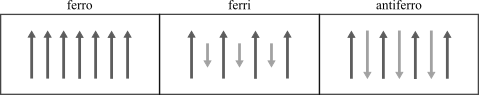
\includegraphics[width=\textwidth]{pictures/magnetic_order.png}
    \caption{Schematic depiction magnetically ordered materials.}
    \label{fig:magnetic_order}
\end{figure}
\FloatBarrier 


\subsection{Domains}
To understand the origin of ultrafast dynamics in magnetically ordered systems we first need to understand what domains are.
They are defined as regions of uniform direction of the order parameter, in the case of ferromagnets it is the magnetization.
This splitting of the magnetic structure into different domains is caused by the minimization of the free energy in the material.
There are several energy contributions coming into play.
Only when they balance out eachother, a stable magnetic state of the sample is possible.
The first and foremost term involved in the forming of domains is the field energy $E_{\text{f}}$ stored in form of the magnetostatic field around the sample.
A large domain also generates a large magnetic field as the field energy scales with the square of the domain size.
Therefore to reduce the field energy the material is split into domains of ever smaller size.
But this shrinking of the domain sizes does not go on indefinetely.
One of the opposing energy terms is the domain wall energy $E_{\text{D}}$ and scales with the root of the domain size.
At the boundries between different domains, which are called domain walls, neighbouring magnetic moments are forced to point in opposite directions.
This goes against the exchange interaction trying to align the magnetic moments in the same direction and there is a energy cost associated with it.
So the domain size is mostly determined by the balance of the field energy saved by domain splitting and the energy cost of additional domain walls.

A further reduction of the field energy is brought on by neighbouring domains having orthogonal magnetizations.
The involved domains are then called flux closure domains.
As the name implies trough the orthogonal arrangement of the domains the field loops get closed almost entirely inside the material.
Since magnetic media have an easy direction of magnetization, flux closure domains result in the magnetization of some domains to be at an angle to this easy direction.
This introduces two additional energetic costs to the equation.
Having the orientation of magnetization at an angle to the easy axis causes an energy term, the magnetocrystalline anisotropy energy $E_{\text{mc}}$, to arise as it is more energetically favourable to have the magnetic moments to align parallel to the easy axis.
The magnetoelastic anisotropy energy $E_{\text{me}}$ is another term caused by a deviation of the orientation of magnetization from the easy axis.
% As a consequence the magnetic dipoles, meaning the ions, deform slightly which induces tiny mechanical stresses on the sample and thus the emerging of such a domain comes with an energy cost.
As a consequence the magnetic dipoles, meaning the ions, deform slightly which induces tiny mechanical stresses on the sample, leading to a phenomenon labeled magnetostriction.
This results in an energy cost hindering the emergence of such closure domains at an angle to the easy axis.

All of these odds in the form of energy costs are stacked against non-parallel alignment to the easy axis which means that most of the volume in a magnetic material holds domains with their magnetization oriented parallel to the easy direction.
This equation
\begin{equation}
    E_{\text{f}} = E_{\text{D}} + E_{\text{mc}} + E_{\text{me}}
    \label{eqn:landau_lifschitz_energy}
\end{equation}
summarizes all the different energy components involved in domain formation.

\subsection{Antiferromagnetic domains}

\section{Magnon dynamics} 


% \section{Sample system NiO/C60}
\section{NiO}
As Ni is a transition metal it carries some unique properties simplifying possible theoretical calculations and making it especially interesting for fundamental research of magnetic materials.
The electronic structure of Ni is $[\text{Ar}]3$d$^8 4$s$^2$.
Entering into a covalent bond with the oxygen 2p-ions the electron configuration of Ni$^{2+}$ changes to $[\text{Ar}]3$d$^8$.
Having a partially filled 3d-orbital in its electronic structure each Ni-ion possesses a net magnetic moment, caused by the angular momenta associated with the unpaired electrons.
Both the orbital angular momentum and the spin of an electron create a magnetic moment.
For a multielectron ion such as Ni$^2+$ with a relatively weak spin-orbit coupling all the angular momenta of each electron couple via the Russel-Saunders coupling.
A big difference to other classes of magnetically ordered elements such as rare earths and actinides is the spatial position of those partially filled shells.
As our object of interest are not single atoms, but crystals containing them, the interaction of the electrostatic crystal field with the orbital motion of the electron is not to be dissmissed.

Rare earths and actinides having their partially filled orbitals (4f and 5f) screened by outer lying shells experience the crystal field interaction as relatively weak or rather just as a small perturbation \lit{Tanner, B. K. (1979)}.
Whereas the transition metals outermost orbitals are exactly those unfilled 3d-shells exposed to the crystal field.
Here, the crystal field is strong in comparison to the spin-orbit interaction.
This leads to their orbital angular momentum being quenched, so that only the magnetic moments of the spin attributes to the net magnetic moment of the ions.

In terms of energy levels the octahedral crystal field exerted by the six neighbouring O$^{2-}$ is responsible for the splitting of the d-states $\Delta_{\text{CF}}$ by lifting the degeneracy in the magnetic quantum number $m_l$.
Additionally an exchange splitting $\Delta_{\text{Ex}}$ takes place depending on the orientation of the spins.
If the exchange splitting is bigger than the crystal-field splitting $\Delta_{\text{Ex}} > \Delta_{\text{CF}}$, as for example in MnO, the spins occupy the lowest possible states, which results in a high-spin state, as seen in \autoref{fig:2}a).
In NiO the exchange and crystal splitting are of similar size and the electrons would occupy a high-spin state as shown in \autoref{fig:2}b) with $S=1$. But even in the case that $\Delta_{\text{CF}}$ would slightly exceed $\Delta_{\text{Ex}}$ the d$^8$-electrons would occupy the same ground state.
Given, the order of the filling would change but the end result would still be the same as with $\Delta_{\text{Ex}} > \Delta_{\text{CF}}$, because the t$_{\text{2g}}$-orbital can contain three electrons and the e$_{\text{g}}$-orbital can contain two electron there is no other way for the d$^8$-electrons to order.
\begin{figure}[ht]
    \centering
    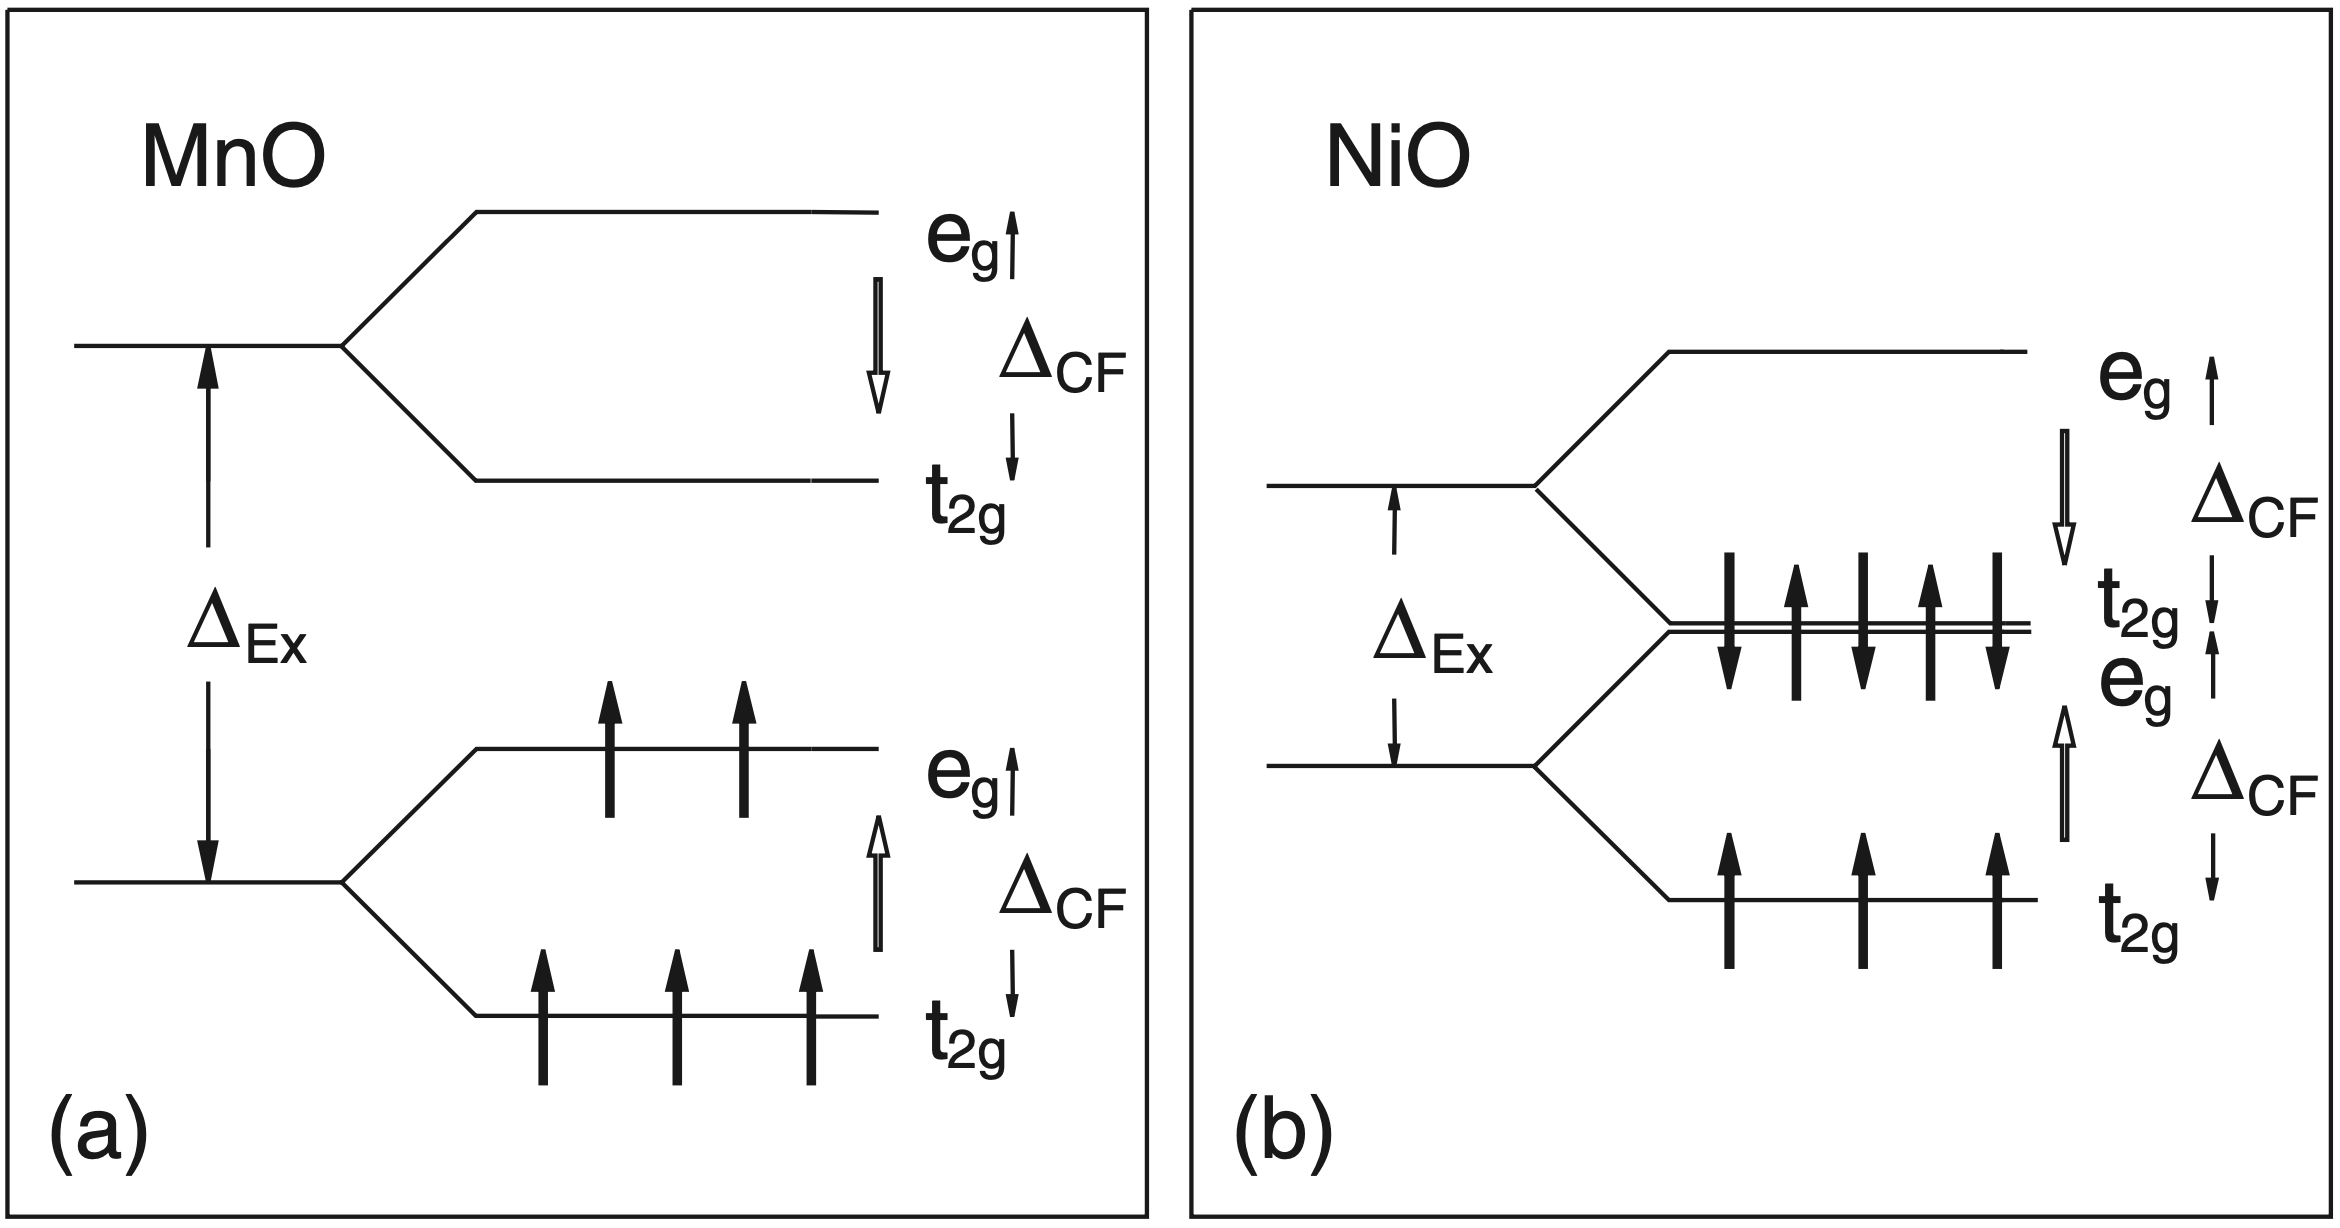
\includegraphics[width=0.8\textwidth]{pictures/2.png}
    \caption{Schema of energy levels of \textbf{(a)} MnO and \textbf{(b)} NiO split by the exchange interaction and by the crystal field. Taken from \lit{B. Fromme}}
    \label{fig:2}
\end{figure}
\FloatBarrier
The one-electron picture including only the Coulomb interactions makes for an intuitive understanding of the occupancy of the ground state, but it does not give the right sizes of the splitting.
The multi-electron picture taking into account the covalency of the 3d-electrons and the 2p-electrons from the oxygen ions and the overlap of the wavefunctions by using the Russel-Saunders terms instead of single electron states.
As the spin-orbit interaction is small the LS-coupling is dominant summing up the angular momenta of each electron s, p, d, ... to the total angular momenta of the whole Ni$^{2-}$-ion S, P, D, ... according to the Hund's rules.
Now the effect of the crystal field on the Russel-Saunders split energy levels of the transition metal ion is calculated.
The crystal field strength $Dq/B$ is taken as a parameter and factors in the Coulomb and also the covalent interaction between the Ni- and O-ions.
Plotting the energy levels against the crystal field strength gives the so called Sugano-Tanabe-diagrams \autoref{fig:4}, which can then be aligned to an absorption spectrum to extract a rough estimate for the crystal field strength, but more importantly to assign experimental results such as absorption edges or transition to the right multiplets.
The result of such an approach is depicted in \autoref{fig:3}.

\begin{figure}[ht]
    \centering
    \begin{subfigure}[b]{0.4\textwidth}
        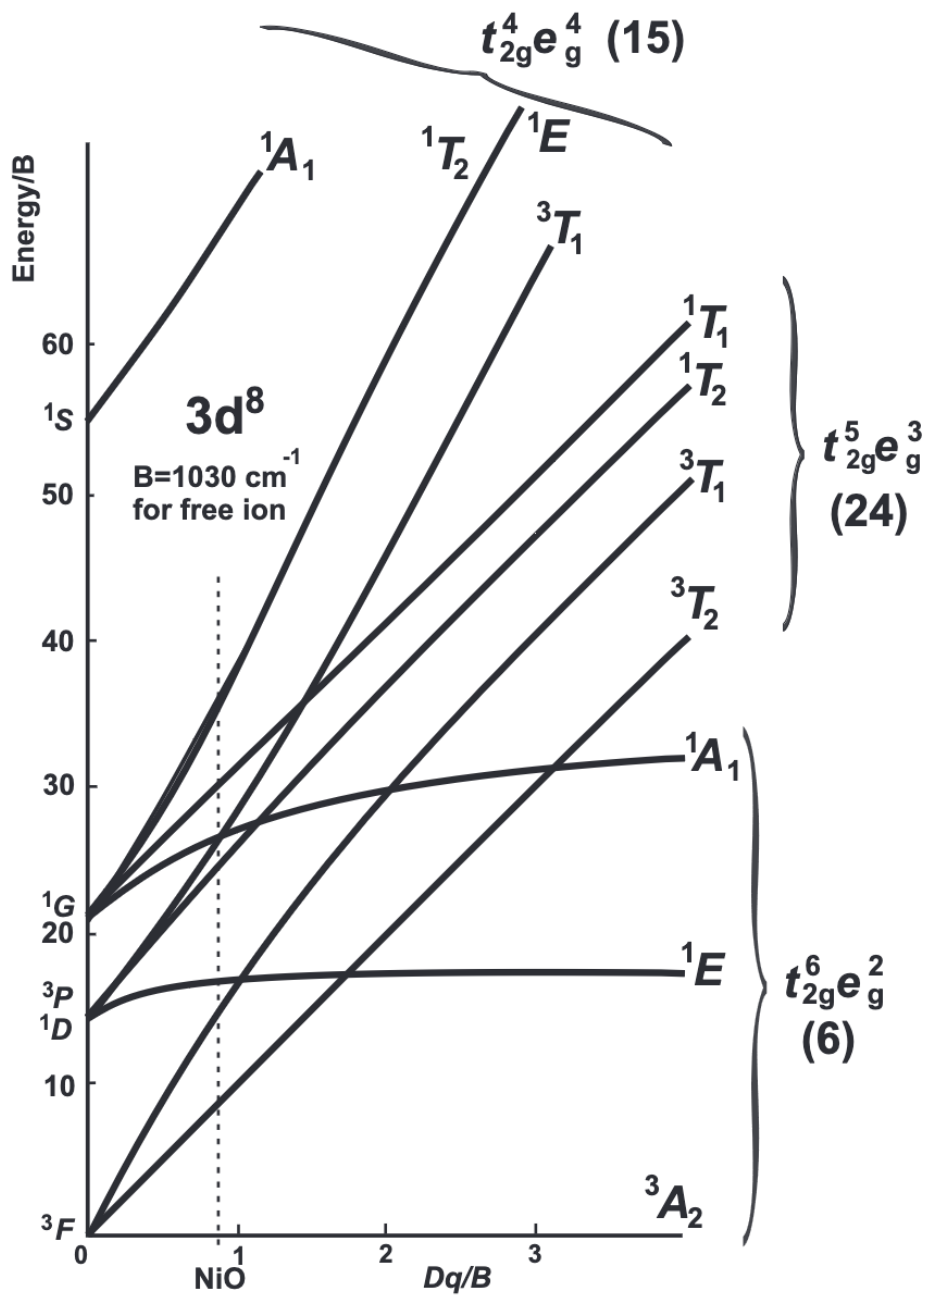
\includegraphics[width=\textwidth]{pictures/4.png}
        \caption{}
        \label{fig:4}
    \end{subfigure}
    \hspace{1cm}
    \begin{subfigure}[b]{0.4\textwidth}
        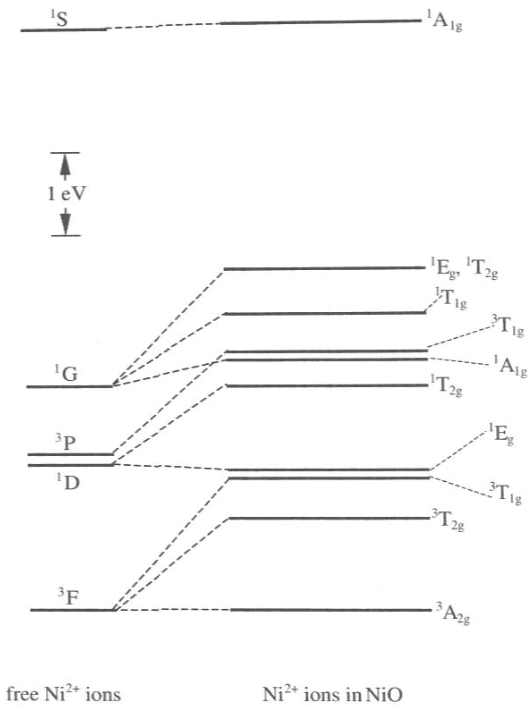
\includegraphics[width=\textwidth]{pictures/3.png}
        \caption{}
        \label{fig:3}
    \end{subfigure}
    \caption{\textbf{a)} The Sugano-Tanabe diagram for Ni$^{2+}$-ions, where the energy levels are plotted against the crystal field strength $Dq/B$. \textbf{b)} The Russel-Saunders terms of the free Ni$^{2+}$-ions on the left and the crystal field splitting of the Ni$^{2+}$-ions in an octahedral field in NiO on the right. Taken from \lit{B. Fromme}}
\end{figure}
\FloatBarrier



\subsection{Magnetic structure}
As mentioned above, the driving force behind the AFM order is the superaxchange between two Ni-ions which are positioned on opposite sites of an O-ion.
In \autoref{fig:1}b its clearly visible that the AFM coupling occurs in one of the $\langle100\rangle$-directions.
The cubic rocksalt structure of the NiO in the paramagnetic phase becomes a rhombohedral one, when going beneath the Neél-temperature of $T_N = \qty{523}{K}$ as the AFM order induces a slight contraction along one of the four equivalent $\langle111\rangle$-axes.
As a result the optic axis also forms along this direction.
In its ordered phase NiO has a cubic anisotropy, meaning two anisotropy directions.
One is the hard axis, where all the atomic spins lie in ferromagnetic sheets in the $(111)$-plane, making it a prototypical easy-plane antiferromagnet.
The magnetization in neighbouring sheets is reversed.
The second one is the easy axis and although it was under some discussion, the consensus now is \lit{Hutchings and Samuelsen; Roth et al.} that the spins point in the $\langle11\overline{2}\rangle$-direction.

Because the rhombohedral contraction can happen along any one of the four equivalent $\langle111\rangle$-axes there exist four twin- or T-domains.
Within these T-domains there are further three equivalent $\langle11\overline{2}\rangle$-axes to which the spins can lie parallel.
These regions of the same spin orientations within the FM sheets are called S-domains, making it a total of 12 possible domains.
Domains can also originate from structural defects, as the strystal structure is tightly connected to the magnetic structure.
Nonetheless, the existence of these domains plays a key role in making the excitation of both magnon modes in NiO possible.
\begin{figure}[ht]
    \centering
    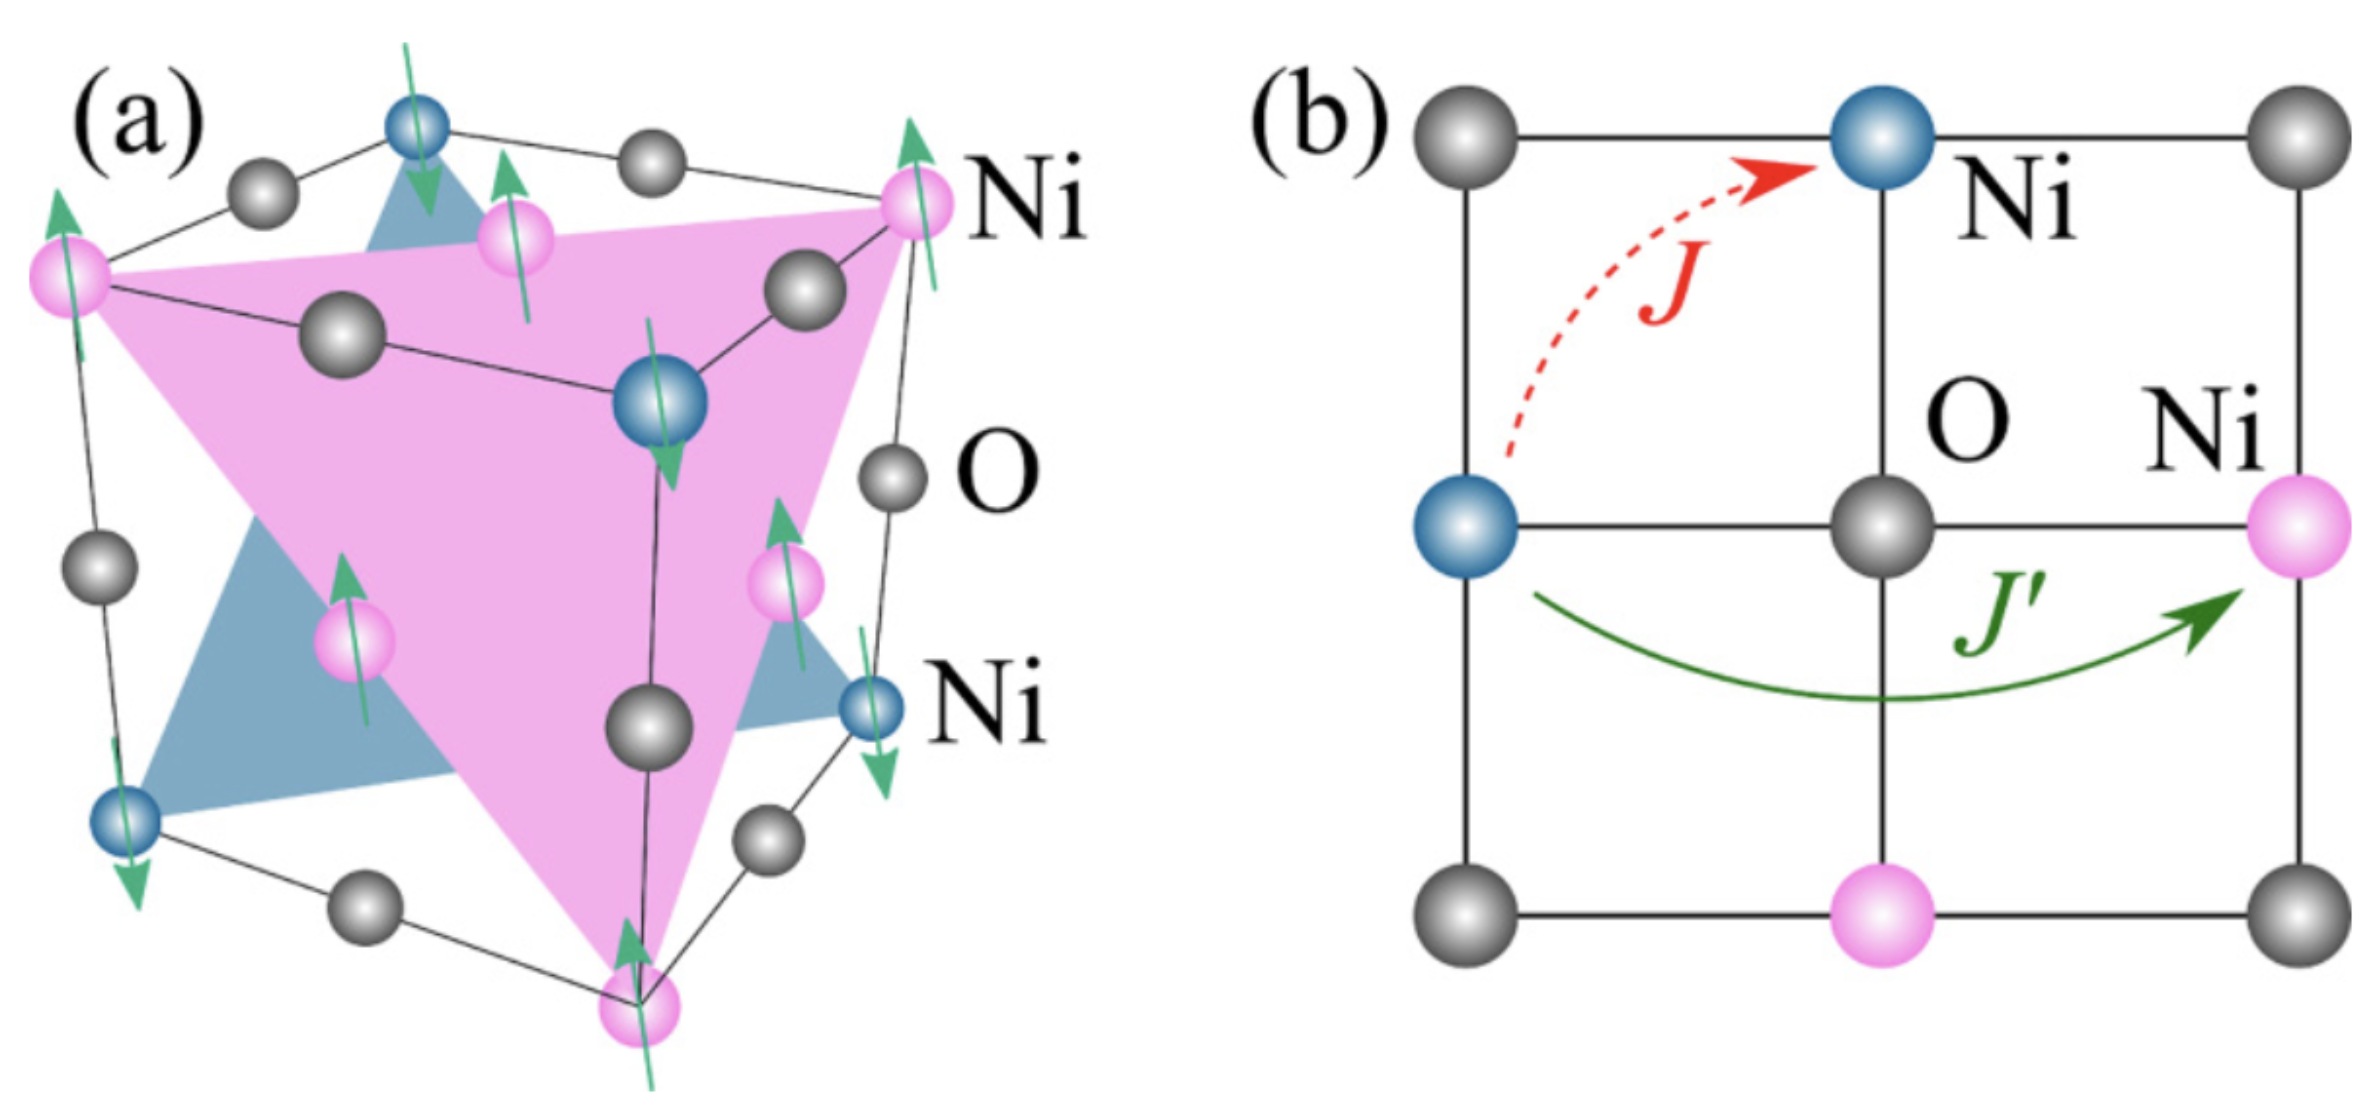
\includegraphics[width=0.6\textwidth]{pictures/1.png}
    \caption{A representation of the crystal and magnetic structure of NiO. Taken from \lit{Betto et al.}}
    \label{fig:1}
\end{figure}
\FloatBarrier

\subsection{Exciton-Magnon-Transition}
\label{sec:x_m}
Many absorption spectra of antiferromagnetic insulators exhibit an additional peak right next to their exciton peaks \lit{Sell} refered to as magnon sideband.
We utilize this exciton-magnon transition to create magnons in NiO.
The exciton peak visible in the absorption spectrum of NiO \autoref{fig:5} at around \qty{0.97}{eV} originates from the spin-forbidden electric dipole d-d transition between the crystal field multiplets $^3A_{2g} \rightarrow \, ^3T_{2g}$.
All d-d transitions in centrosymmetric environments, such as the octahedral one of the Ni$^{2+}$-ions, are parity forbidden by the Laport rule $\Delta L = \pm 1$.
This selection rule is easily explained when you consider the symmetry of the the initial wavefunction $\Psi_i$, the final wavefunction $\Psi_f$ and the transition moment operator $\mu$, when looking at the transition matrix element
\begin{equation}
    M_{if} = \int_{\mathbb{R}^3} \Psi^*_f \cdot \mu \cdot \Psi_i \;\text{d}r^3 \;.
    \label{eqn:laport}
\end{equation}
For the matrix element to be non-zero when integrating over the whole euclidian space the product $\Psi^*_f \cdot \mu \cdot \Psi_i$ inside the integral in \autoref{eqn:laport} has to have an even parity.
For electric dipole transitions the $\mu$ is odd, so that a transition is only allowed if the initial and final wavefunction are of different parities totaling to an odd parity.
What breaks the inversion symmetry in NiO and what allows for the d-d transition to happen is the silmultaneous creation of a magnon.
For an intuitive understanding you could think of this in the same way as thinking of a phonon with an odd vibration breaking the centrosymmetry and thus allowing d-d transitions showing itself as a phonon sideband.
The spin-forbideness is also lifted by the magnon as it compensates the spin, which is only possible and also why we only see this in antiferromagnets.
\begin{figure}[ht]
    \centering
    \begin{subfigure}[b]{0.3\textwidth}
        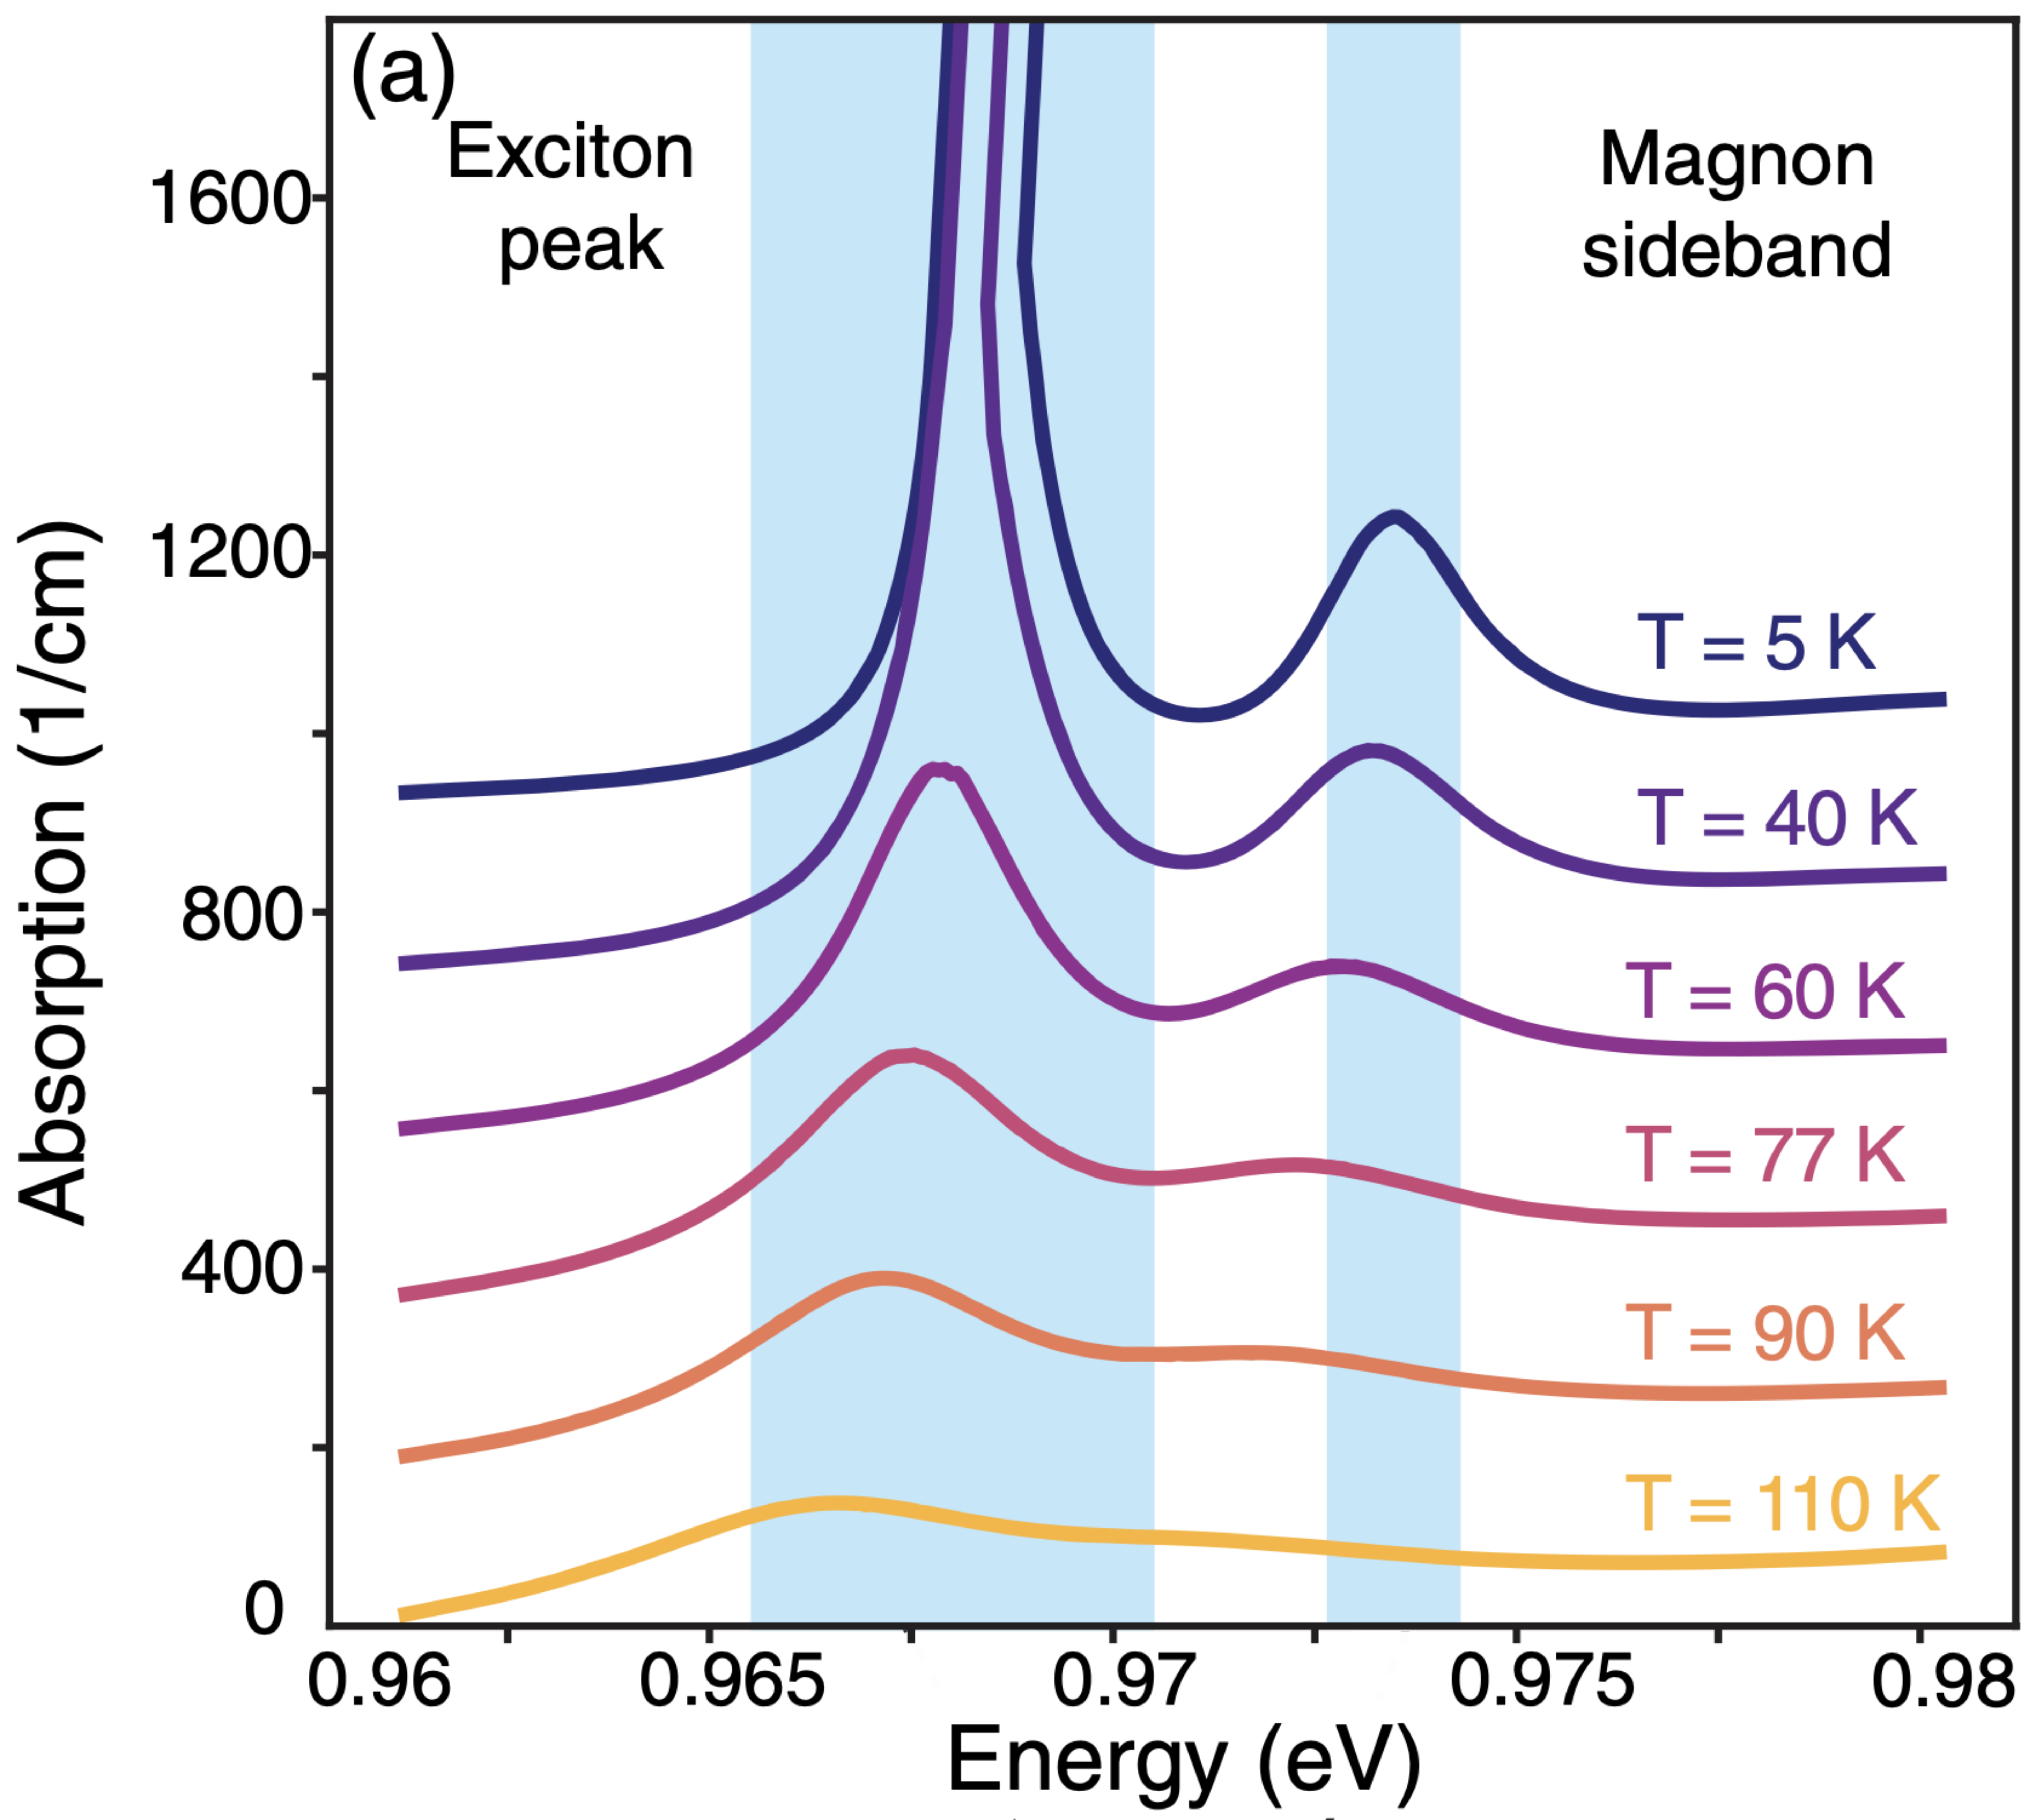
\includegraphics[width=\textwidth]{pictures/5.png}
        \caption{}
        \label{fig:5}
    \end{subfigure}
    \hspace{1cm}
    \begin{subfigure}[b]{0.6\textwidth}
        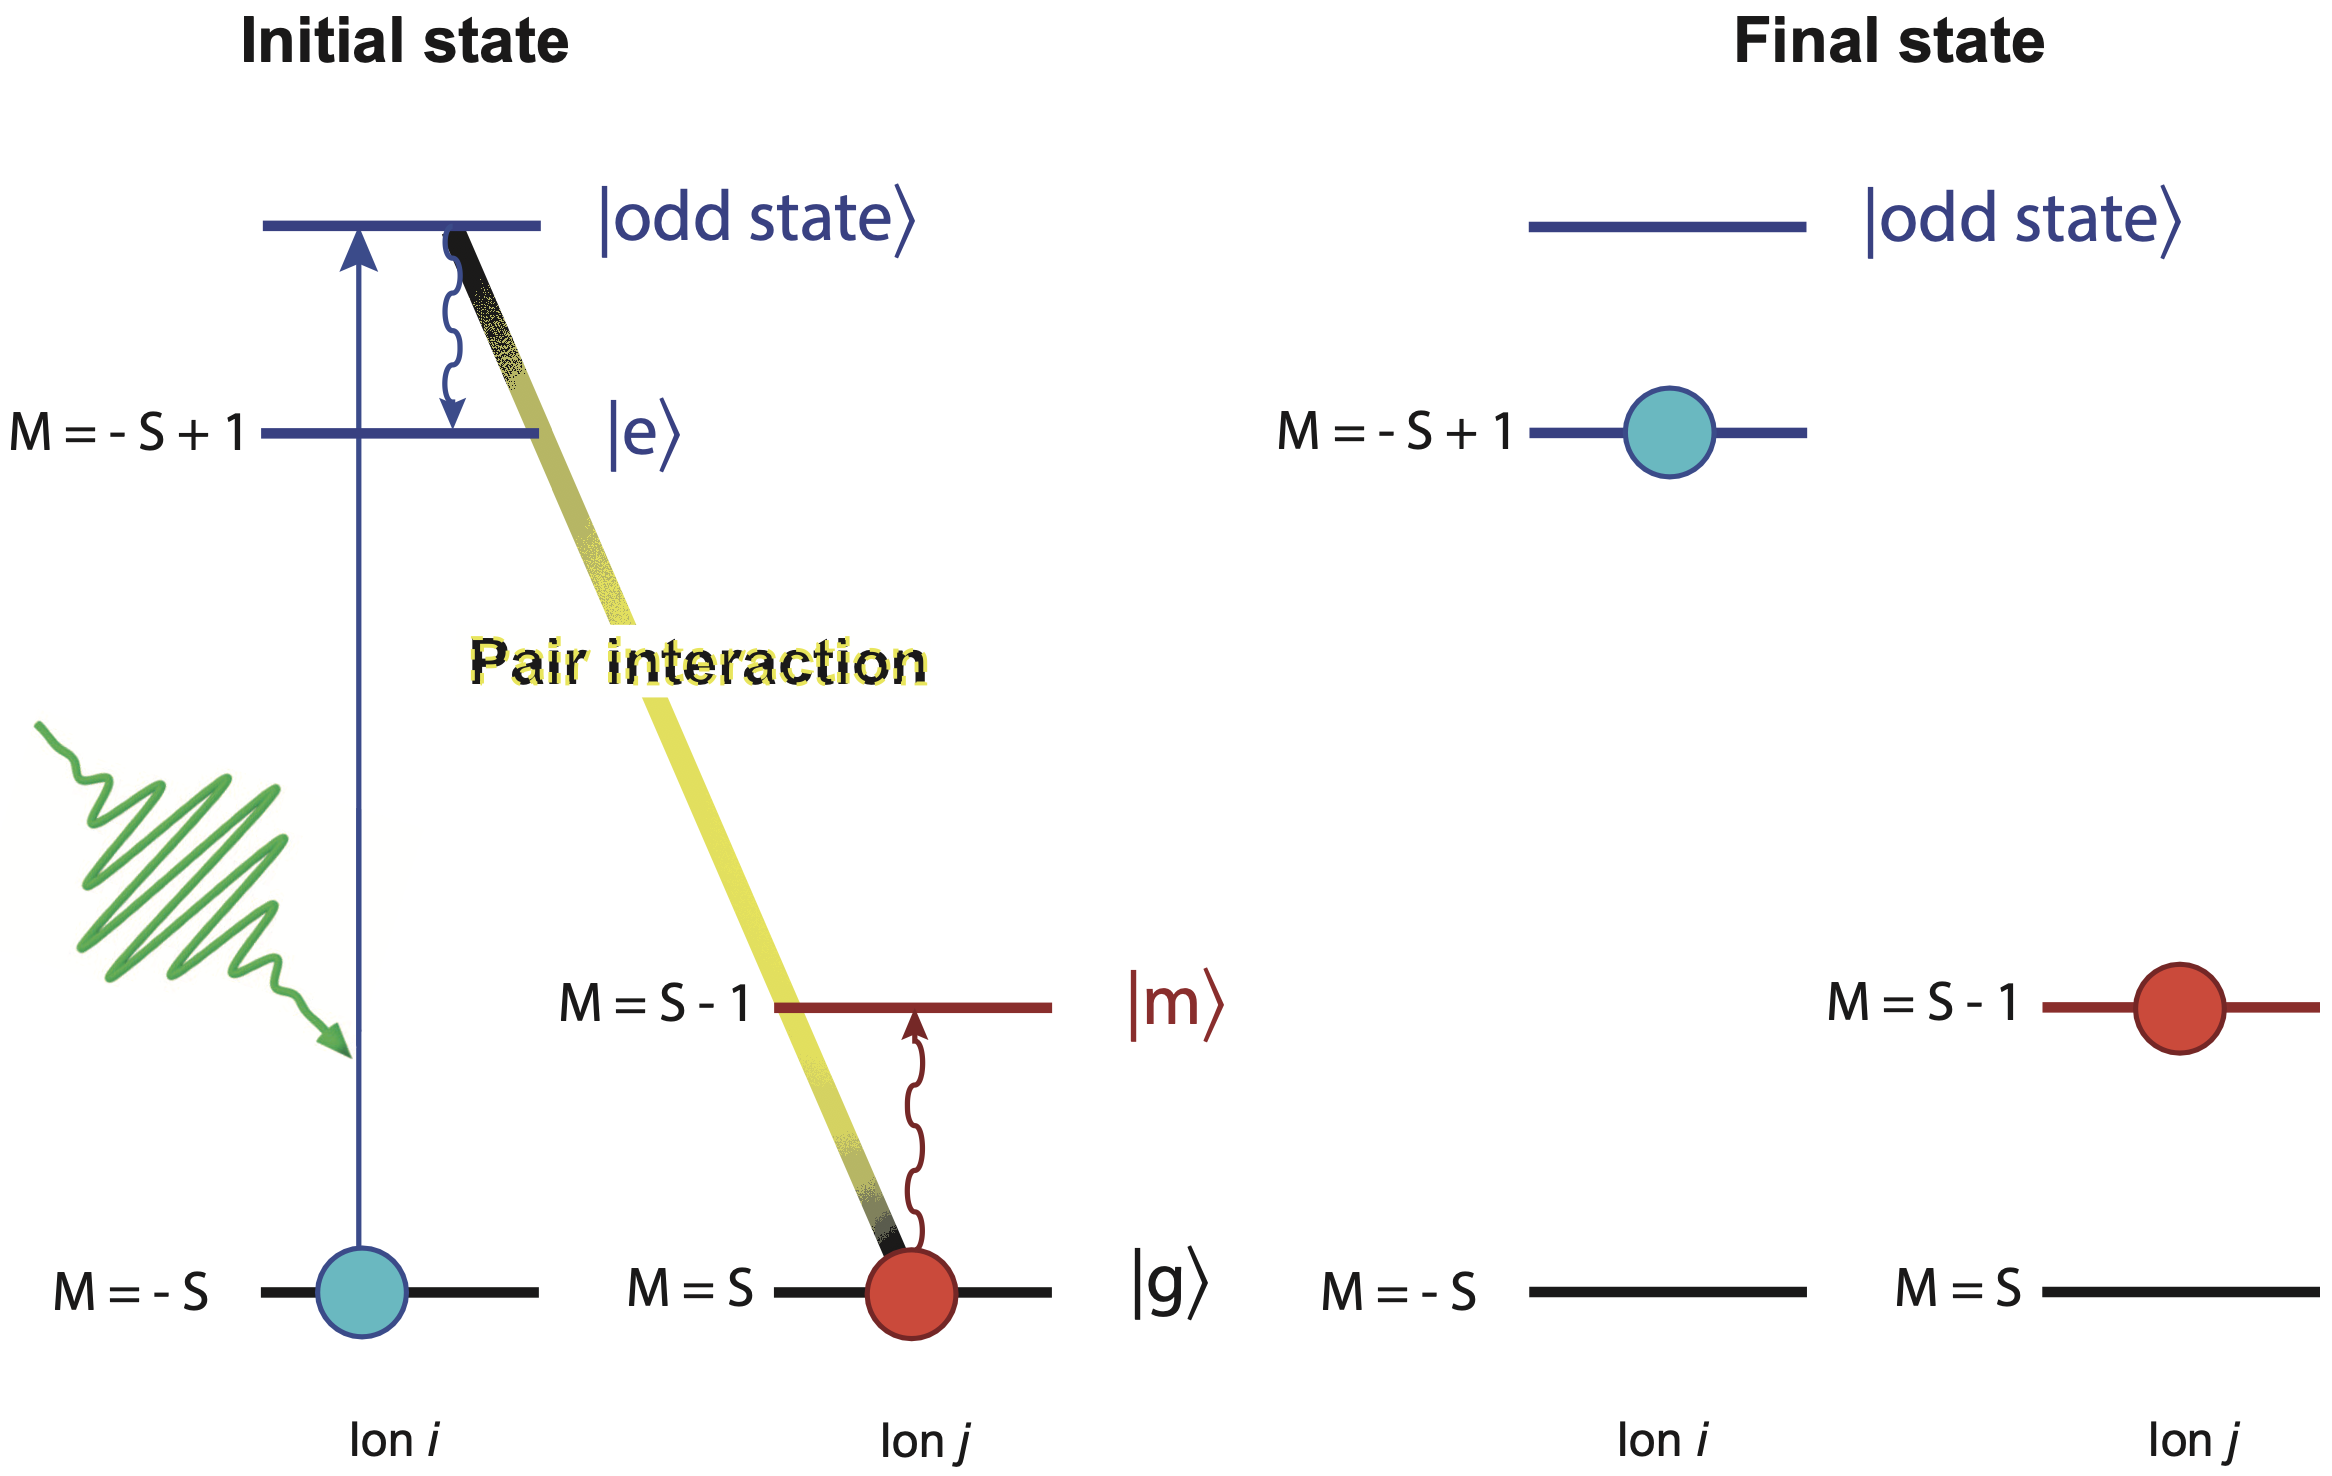
\includegraphics[width=\textwidth]{pictures/6.png}
        \caption{}
        \label{fig:6}
    \end{subfigure}
    \caption{\textbf{a)} The absorption of NiO in the energy range around the exciton-magnon resonance, measured at different temperatures. \textbf{b)} A schematic representation of the energy levels and transitions involved in the exciton-magnon transition. Taken from \lit{Bossini et al.}}
\end{figure}
\FloatBarrier
\autoref{fig:6} shows a schematic diagram on the basis of which the explanation of the concrete process behind the exciton-magnon transition is easier to follow.
Two Ni$^{2+}$-ions, each from one of the two sublattices, are involved in this scheme.
First, a photon hits the 1. ion with spin $-S$ and raises it into an opposite parity state compared to the ground state, which is odd since the ground state is taken as even.
This electron excitation is described as a Frenkel exciton, because the spatial extensions of the involved d-orbital are small compared to the lattice parameter, which is exactly the case for the tightly bound 3d-electron in the Ni-ions.
The ion relaxes to its final state $|e\rangle$ with even parity, but undergoing a change in spin to $-S+1$.
Silmultaneously, mediated by the superexchange interaction between the two ions, the 2. ion in the other sublattice with spin $S$ undergoes an electric-dipole transition to a state $|m\rangle$ with spin $S-1$.
These two spin-changing transitions are only possible, because they happen at the same time and the total spin is conserved.
Frenkel excitons with a change of spin are essentially spin waves, so this whole process effectively created a magnon mode causing the precession of spins in both sublattices.

\subsection{Magnon coupling}
\label{sec:mode_coupling}
Theory predicts different AFM resonance modes depending on the model used to simulate the dispersion and magnetic or temperature dependencies.
They contain different interactions and different amounts of sublattices.
A two-lattice model is best used to describe the two magnon modes at the Brioullin-zone center with frequencies of \qty{1.07}{THz} and \qty{0.13}{THz} visible when pumping with light in the infrared region.
Apparently
There is also a 8-sublattice model predicting five different degenerate modes at $k=0$ 

\section{C60}





% \chapter{Experimental setup}
As this thesis deals with the manipulation of the magnetization of antiferromagnets via optically driven thermal and electronic excitations \cite{song_how_2018} the observed dynamics take place on the ultrafast timescale and a time-resolved technique capable of femtosecond resolution is needed.
This is achieved using a pulsed femtosecond laser.
All measurements are carried out using the table-top setup as established by Mertens et al. \cite{mertens_wide_2020}.

\subsubsection*{Pump-probe measurements}
In the frame of this thesis most of the measurements are done via pump-probe spectroscopy, as we focus on the ultrafast time evolution of the antiferromagnetic systems after an optical excitation.
Two pulsed laser beam are used to take time resolved measurements, the pump and the probe.
The pump pulse acts as a perturbation and excites the system causing a change in its ordered structure.
The probe pulse is used to probe the perturbed system and to extract information about the origin of the change, which translates to a MO effect happening in turn causing measurable modification of the probe pulse such as the rotation of polarisation or ellipticity.
By shifting the time delay between these two laser pulses it is possible to figuratively scan the system's response in the time domain.
A delayline with a minimal stepsize of \qty{75}{nm} in the pump path enables the control of the time delay down to \qty{50}{fs} limited only by the pulse duration itself.
\begin{figure}[ht]
    \centering
    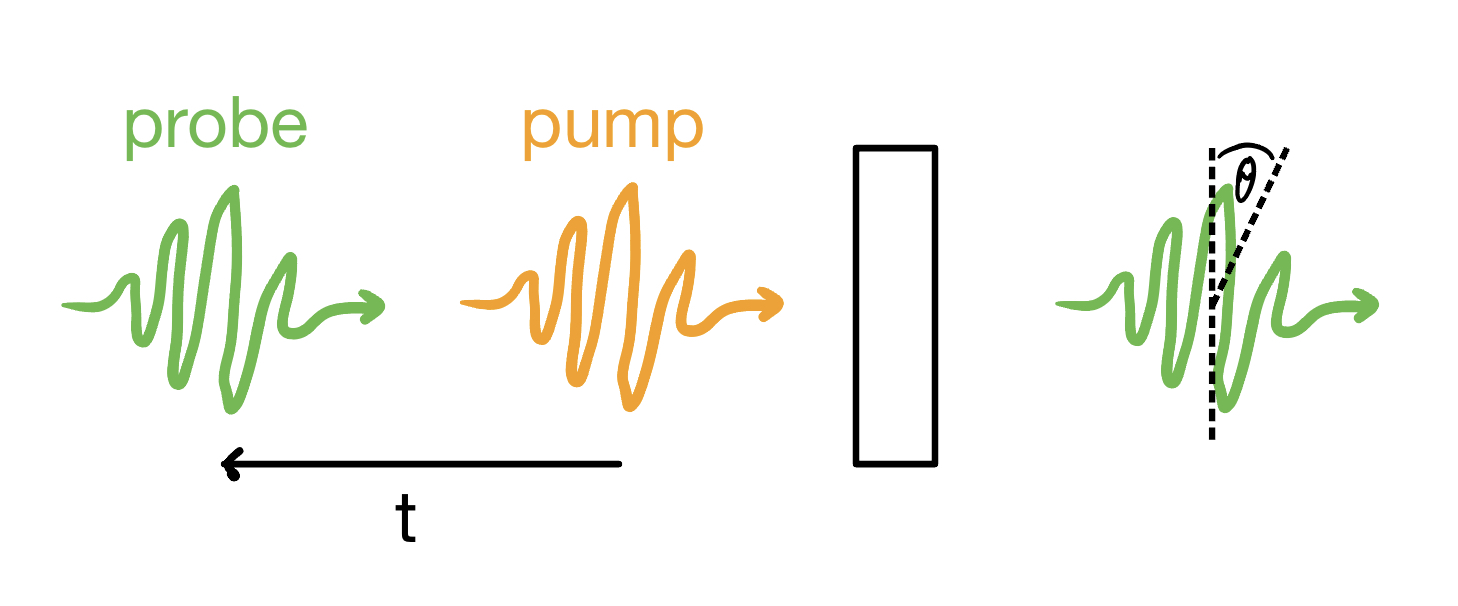
\includegraphics[width=0.6\textwidth]{pictures/pump_probe.jpeg}
    \caption{Schematic depiction of transmission pump-probe measurement.}
    \label{fig:pump_probe}
\end{figure}

\subsubsection*{Laser system}
Here a commercial ytterbium-based pulsed femtosecond laser (PHAROS) made by Light Conversion with a central wavelength of \qty{1028}{nm}, a pulse duration of about \qty{300}{fs} and a power of \qty{20}{W} is used.
With a repetition rate of \qty{50}{kHz} each pulse carries an energy of \qty{100}{\uJ}.
The Pharos output is split into two beams with \qty{7}{W} and \qty{13}{W}, of which the first one is designated to be the probe and the second to be the pump beam.
To ensure a separate tunability in wavelength of the two beams each one is fed into an optical parametric amplifier (OPA) Orpheus.
The OPA consists of a series of non-linear optics mounted on motorized stages, containing among others white light generation (WLG) and difference frequency generation (DFG).
The former of which makes it possible to select a specific signal frequency to amplify via the DFG process.
\begin{figure}[ht]
    \centering
    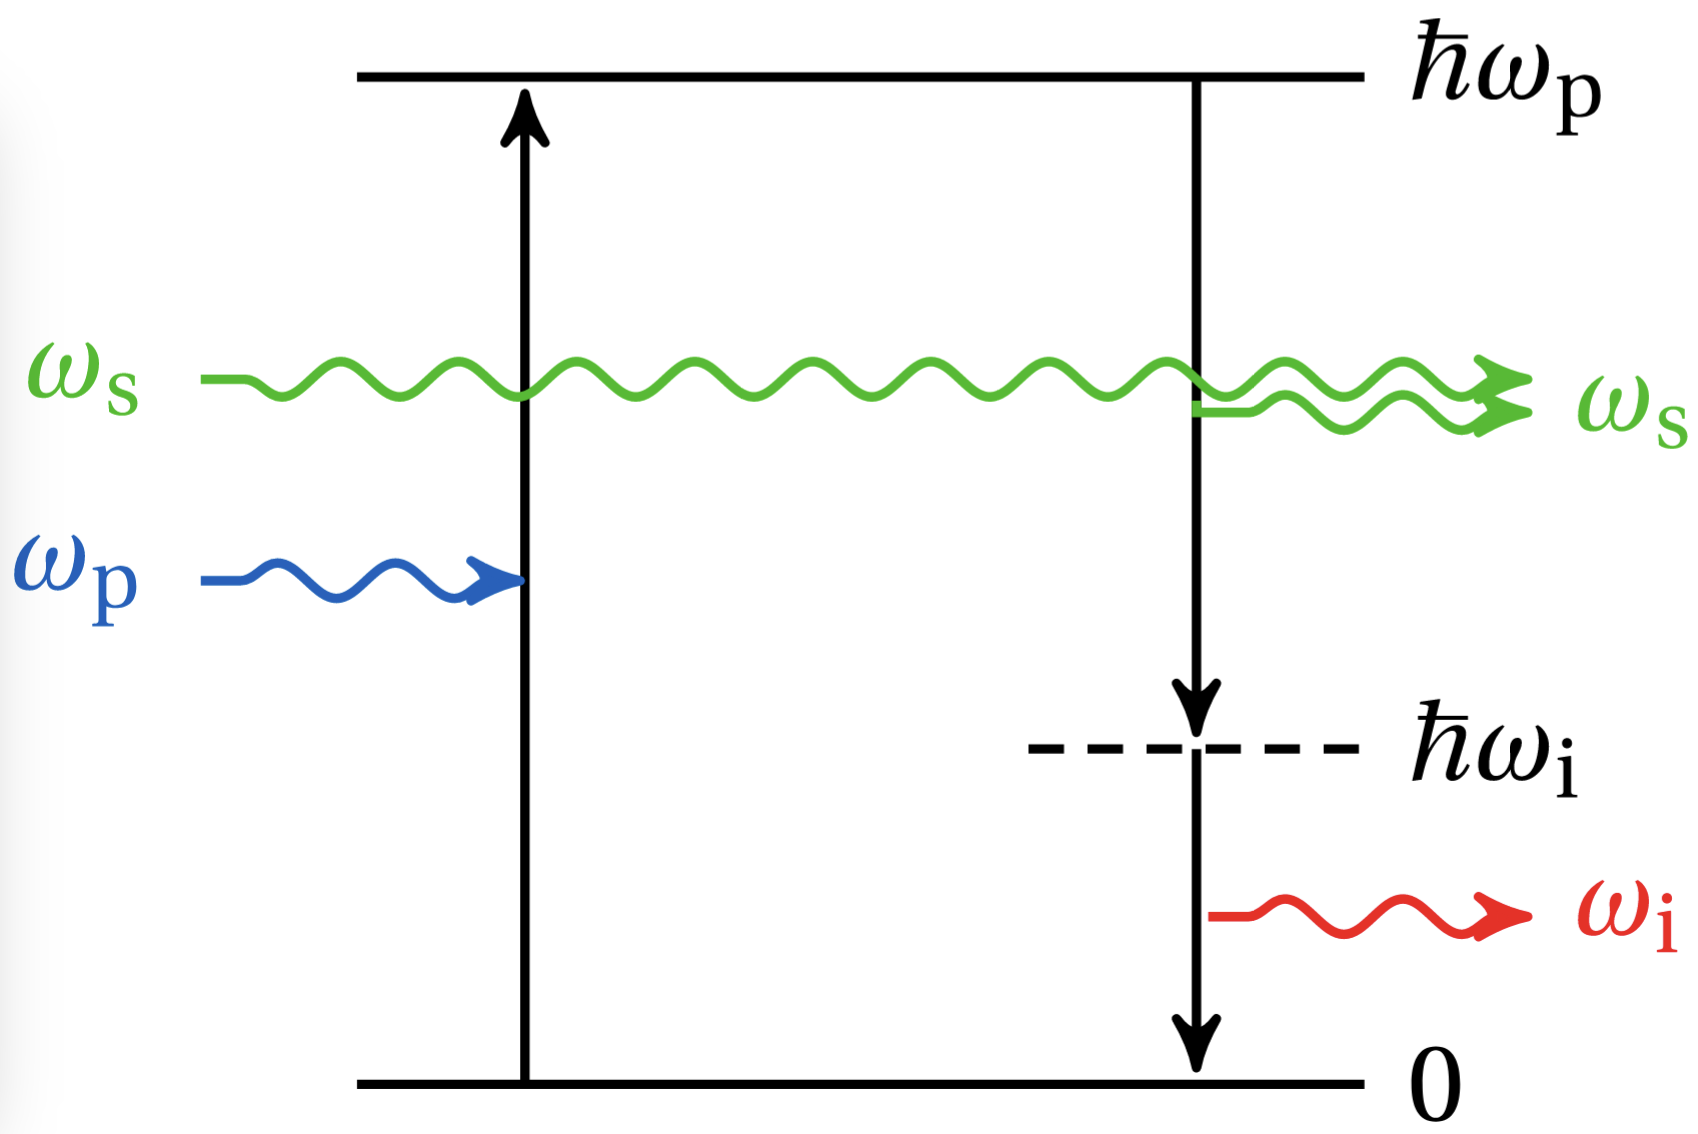
\includegraphics[width=0.5\textwidth]{pictures/OPA.png}
    \caption{Illustration of energetic transisions involved in the process of optical parametric amplification.}
    \label{fig:OPA}
\end{figure}
As can be seen in \autoref{fig:OPA} a pump beam is necessary to amplify the signal beam.
Another beam called idler is created as a byproduct, so that the following relation holds:
\begin{equation*}
    \omega_{\text{p}} = \omega_{\text{s}} + \omega_{\text{i}}
\end{equation*}
Before the OPA for the pump an electro optical modulator is placed only letting every second pulse pass.
This has the effect that half of the probe pulses encounter an unpumped sample, which sets a baseline for the detected signal.
The OPA also incorporates an internal compressor for the idler beam.
To compensate for the signal beam, its path can be manually adjusted via a quick replacement of mirrors to go through an external compressor.
Making up the last component of the stationary laser system is the external second harmonic generator (LYRA).
It extends the spectrum by twice reaching from \qty{0.5}{eV} to \qty{3.5}{eV}. 
\begin{figure}[ht]
    \centering
    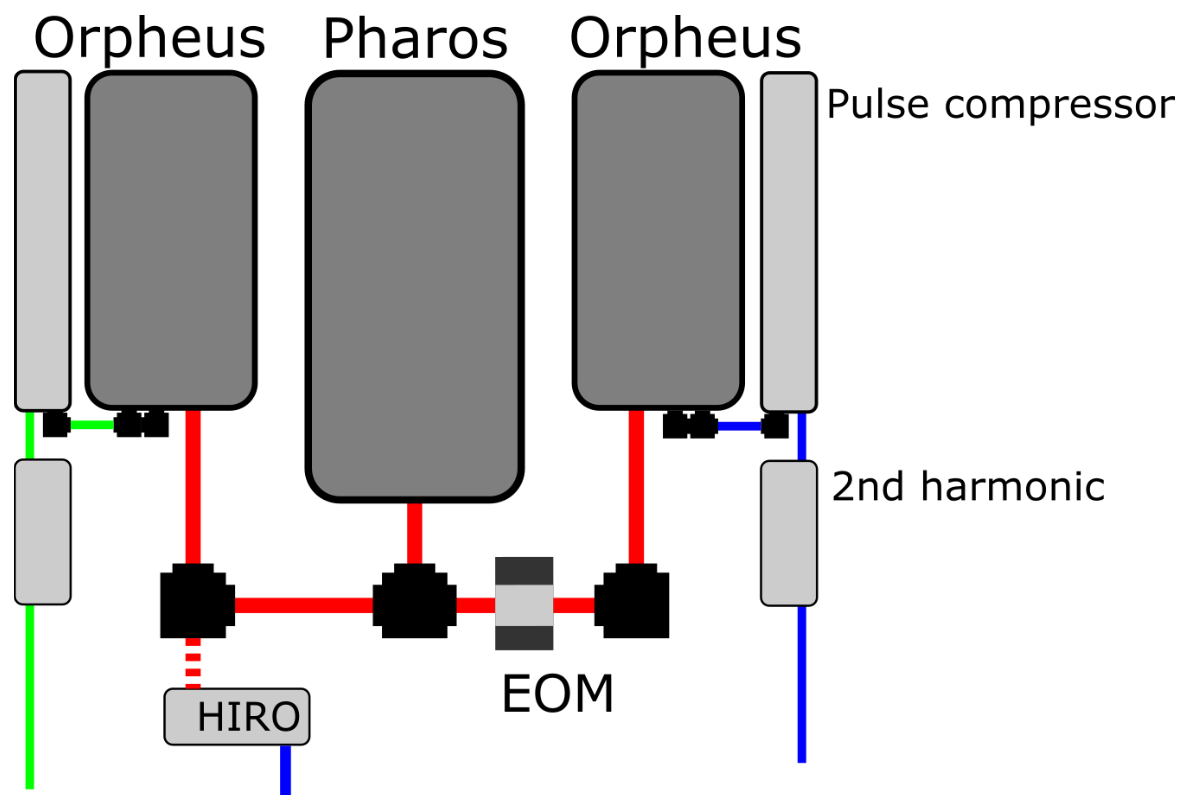
\includegraphics[width=0.65\textwidth]{pictures/laser_system.png}
    \caption{Schematic of the laser system containing labelled parts.}
    \label{fig:laser_systems}
\end{figure}
With the exception of the external compressor, the system can be operated with the corresponding desktop application and automatically adopts the typed-in wavelength.

\subsubsection*{Optical path}
As already mentioned above, a delayline is stationed in the pump beam path.
The pump travels the distance between the mirror and the delayline four times, which accounts for a factor of $\frac{4}{c}$ between the time delay and the shifted distance.
The laser light is horizontaly polarized to the plane of the table [PHAROS manual], so as an attenuator for the high peak power, a linear polarizer cube in combination with a $\frac{\lambda}{2}$-waveplate is used.
To vary the transmitting intensity the waveplate is rotated and to vary the angle of the light polarization for polarization dependent measurements an additional $\frac{\lambda}{2}$-waveplate is installed behind the attenuator.
Both the beams are then focused either by lenses or an objective on a common point on the sample surface, where a spatial overlap is achieved by using the computer-controlled piezo-driven mirror-holder from Newport.
% It is possible to use this system in the collinear, pump and probe are parallel, or the transversal, angle between pump and probe, scheme.
% The decision which geometry to incorporate is made based on the direction of the anisotropy.
Furthermore the setup can be adjusted for reflective or transmissive measurements.
The transmissive measurements being the more straightforward ones to implement wheras the reflective ones require the use of a beamsplitter to guide the light to the detection branch.

The sample is mounted in a open-loop cryostat requiring a steady flow of helium to reach and hold a desired temperature, which is essential for measurements exploring phase diagrams.
A magnetic valve controls the cross section of the supply pipe and thus the quantity of helium being pumped through the cryostat.
To maintain a specific steady temperature a heater governed by a PID controller is in thermal contact with the sample holder.
The cryostat itself is inserted inside a closed-loop, helium-cooled, superconductive magnet generating up to $\pm\qty{9}{T}$ at the sample position normal to the sample plane.
This allows for magnetic field dependence measurements, as well as for recording of hysteresis curves.
The sample stage has three axis and can be computer-controlled down to a stepsize of \qty{1}{nm} to shift to an exact position.

\subsubsection*{Data aquisition system}
MO effects typically induce a rotation of the polarization or ellipticity in the incident light and as most of the observed samples in the context of spintronics are rather thin, the change in the probe light often amounts to only a few mrad.
To overcome this issue, a specialised technique called balanced photodetection is used suppressing the background noise while simultaneously amplifying the difference between two incoming optical signals.
Firstly, the reflected or transmitted probe beam is guided through a $\frac{\lambda}{2}$-waveplate and a Wollaston prism.
The prism splits the light $I$ in two linearly polarized rays $I = I_p + I_s$ with their polarizations perpendicular to each other as depicted in \autoref{fig:balanced_detection}.
\begin{naligned}
    E_s &= E \cos\left(\sfrac{\pi}{4} + \theta\right) \\
    E_p &= E \sin\left(\sfrac{\pi}{4} + \theta\right)
    \label{eqn:balance}
\end{naligned}%
The waveplate is used to tilt the polarization of the light to such a degree that both of the rays hit the photodetector with the same intensity.
From this equilibrium position with a now switched on, previously arriving pump pulse, the polarisation of the probe gets rotated by an angle $\theta$.
This changes the ratio between the two photocurrents, which get converted into voltage and whose difference then gets amplified via operational amplifiers.
\begin{figure}[ht]
    \centering
    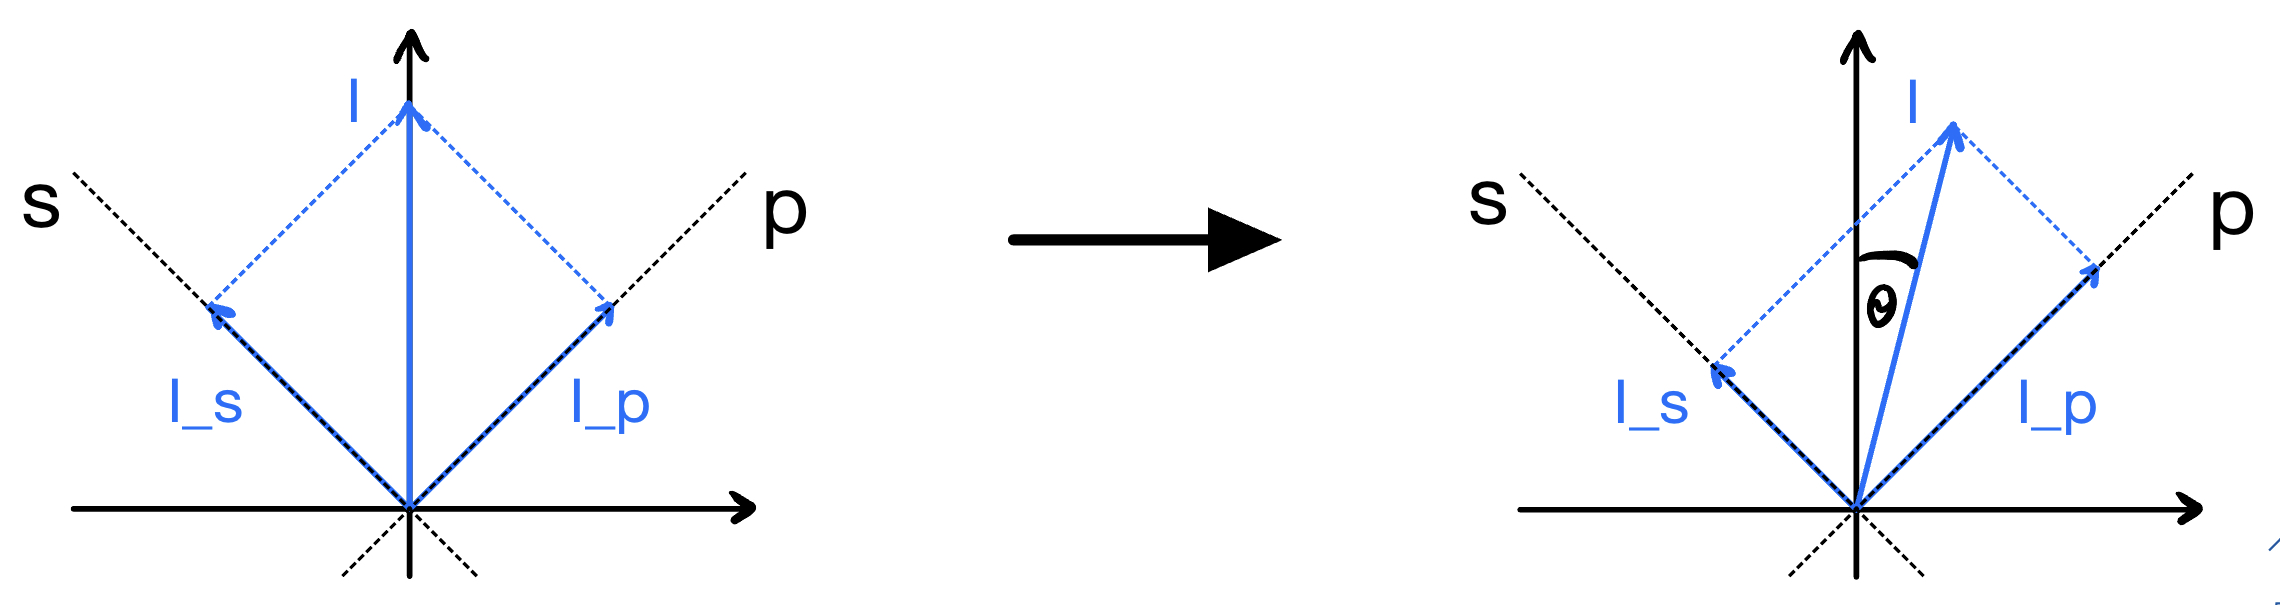
\includegraphics[width=\textwidth]{pictures/balanced_detection.jpeg}
    \caption{Representation how the incoming light gets split by the prism into two equally intense linearly polarized rays and how the subsequent rotation of polarisation materializes in the difference between s- and p-polarized light intensity.}
    \label{fig:balanced_detection}
\end{figure}
As the light is measured with a photodetector the incident light power is proportional to the generated current which in turn is proportional to the converted voltage and thus the signal observed on the computer.
Using this and \autoref{eqn:balance} the proportional  relation
\begin{equation}
    S \propto E_s^2 - E_p^2 \approx 2 E^2 \theta
\end{equation}
between a small angle $\theta$ and the signal $S$ can be derived.
% \chapter{Results and discussion}
\section{Exemplary analysis of pump-probe trace}
The analysis of the pump-probe time traces was either done by fitting the data or by applying a fast fourier transform (FFT).
We can measure and analyze the rotation of polarization as the normalized difference between the two photodiode inputs and the transient reflectivity as the sum of the two photodiode inputs.
In \autoref{fig:example_analysis_fit}b we use a suitable dataset of rotation of polarization to demonstrate both of these methods.
\begin{figure}[ht]
    \centering
    \includegraphics{pictures/plots/example_analysis_fit.pdf}
    \caption{\textbf{a)} An example trace analyzed using the fitting functions \autoref{eqn:fit_hf} and \autoref{eqn:fit_lf}. \textbf{b)} After subtracting a linear background an FFT was applied, producing this plot.}
    \label{fig:example_analysis_fit}
\end{figure}
\FloatBarrier
The upper part of \autoref{fig:example_analysis_fit}a shows the data as well the first "lf-fit", indicated by a solid red line, done to extract the frequency $f_{\text{lf}}$ and amplitude $A_{\text{lf}}$ of the lower frequency mode by fitting
\begin{equation}
    f(t) = A_{\text{lf}} \cdot \exp(-\lambda_{\text{lf}} t) \cdot \cos(2 \pi f_{\text{lf}} t + \phi_{\text{lf}}) + C \cdot \exp(-\lambda t) + D \cdot x + E
    \label{eqn:fit_lf}
\end{equation}
to the data.
$\lambda_{\text{lf}}$ represents the decay constant of the lf-oscillation and $\phi_{\text{lf}}$ is its phase.
From the viewpoint of the higher frequency mode the lower frequency mode resembles more of a background which is why any exponential and linear contributions to the background are also included in \autoref{eqn:fit_lf}.
% In relation to the higher frequency mode the lower frequency mode resembles more of a background which is why any exponential and linear contributions to the background are also included in \autoref{eqn:fit_lf}.
After subtracting the GHz-fit from the data the simpler fit function
\begin{equation}
    f(t) = A_{\text{hf}} \cdot \exp(-\lambda_{\text{hf}} t) \cdot \cos(2 \pi f_{\text{hf}} t + \phi_{\text{hf}}) \;,
    \label{eqn:fit_hf}
\end{equation}
only featuring an exponentially decaying sine-wave, is used to extract the frequency $f_{\text{hf}}$ and amplitude $A_{\text{hf}}$ of the hf-mode.
This fit is depicted in the lower part of \autoref{fig:example_analysis_fit}a by the red line.
The results of both fits are shown in \autoref{fig:example_analysis_fit}b as the red markers.

Since the only important parameters in the context of this thesis are the amplitude and the frequency of the modes, the FFT represents another approach for the data analysis.
Here, only the background is fitted in preparation for applying the FFT, so that the oscillations are singled out and so that they can be broken down into a linear combination of sine or cosine functions, as is the premise of a fourier transform.
A discrete fourier transform of a perfectly sinusoidal signal yields an infinitely thin peak at one exact frequency.
The exponential decay of the oscillation in the time-domain translates to a finite width of the resulting peak in the frequency domain together with a reduction in the height of the peak.
This effect is called dephasing and happens because the amplitudes get redistributed over more frequency bins, as the uncertainty rises.
The faster the decay happens, the wider the peak gets, as you can see in \autoref{fig:example_analysis_fit} for both of the modes.
The peak of the FFT associated with the lf-mode is much lower than the amplitude acquired through the fit.
The peak of the hf-mode is also slightly lower than the amplitude of the fit which is also attributed to the same effect, albeit to a smaller extent.

But more importantly, if no decay is visible in the observed time interval, this effect can be neglected.
In view of this, the fitting method is used to analyze the measurements on NiO/C60, as a clear decay is visible there.
The FFT method is used for the measurements of NiPS3, since no decay of the oscillations is discernable.


\section{NiO/C60}
\subsection{Absorption measurements on NiO/C60}
As described in \cite{rezende_introduction_2019}, NiO is as a prototypical antiferromagnet which was already a subject of much research effort.
In this thesis we focus on the changes we can detect in the magnetic behavior by covering the NiO with a molecular layer.
To try this, C60 was used in part because it is widely available, but mainly because of its strong interaction with ferromagnetic surfaces \cite{veenstra_interface_2002}.
% C60 is a molecule which is
% (strong surface dipole formation) when in contact with () ..... 
Assuming that C60 changes the magnetic anisotropy which has a direct influence on the magnon frequency in NiO it is adsorbed on its surface.
\begin{figure}[ht]
    \centering
    \includegraphics[width=0.7\textwidth]{pictures/plots/NiO_absorption_nm.pdf}
    \caption{Absorption spectra measured on the CARY system at \qty{4}{K} for pure NiO (blue line) and for NiO/C60 (red line). The lower part is a zoom-in on the d-d transition.}
    \label{fig:NiO_absorption_nm}
\end{figure}
\FloatBarrier
Ahead of the time-resolved measurements, static absorption spectra were acquired at \qty{4}{K} using the commercial spectroscopy Cary 6000i system by Agilent.
Two \qty{15}{\mu} thick NiO samples were measured, one pure NiO sample and one NiO sample with the adsorbed C60-molecules.
\autoref{fig:NiO_absorption_nm} shows the absorption spectra of both of the samples in the range of 1000 to \qty{1500}{nm}.
As the two samples did not have the same size, a direct comparison of the two spectra by subtraction or division was not possible.
Nonetheless, an obvious broadening of the exciton peak at \qty{1280}{nm} and the magnon-sideband at \qty{1273}{nm} is visible in the spectrum of NiO/C60 in \autoref{fig:NiO_absorption_nm}, especially in the zoomed-in view on the bottom.
While still being distinct, the exciton-magnon (X-M) peaks of NiO/C60 seem to have shifted slightly to higher energies by about \qty{1}{meV} with respect to the ones froms the pure NiO.
Furthermore, some additional features between \qty{1350}{nm} and \qty{1400}{nm} are clearly visible in the spectrum of the NiO/C60 in contrast to the one from the pure NiO and may be worthwhile to examine.

\subsection{Pump wavelength dependence of NiO/C60}
A pump wavelength dependence around the X-M peak (\qty{0.97}{eV}) on pure NiO has already been performed by Bossini et al. \cite{bossini_ultrafast_2021} which is also featured here and which some of the following explanations are based on.
Now we want to see what impact the hybridization of the pure NiO surface with the C60 molecule layer has on the domain structure and thus on the coupling of the two magnon modes.

The pump wavelength dependence consists of measurements taken at different pump wavelenghts ranging from \qty{1158}{nm} to \qty{1362}{nm}, which are shown in \autoref{fig:NiO_pump_WL_dependence}.
The traces cover a time interval of around \qty{25}{ps} ensuring that they encompass at least three whole periods of the lf-mode each lasting \qty{7.7}{ps}.
The start of the cross-correlation was taken as the zero point in the plot.
To extract the frequency and amplitude of the lf-oscillations the data was fitted using the fit function \autoref{eqn:fit_lf}.
The fits are indicated by the red lines in the plot. 
Due to the absence of any lf-oscillations, it was not possible to fit the two uppermost traces and thus no red lines were plotted along them.
After subtracting the fits of the hf-mode from the initial data we get the plots featured in \autoref{fig:NiO_pump_WL_dependence_THz}.
Now only the hf-oscillations remain and thus an exponentially decaying sine-wave \autoref{eqn:fit_hf} is used to fit the data, which is again indicated by the red lines.
\begin{figure}[ht]
    \centering
    \includegraphics{pictures/plots/NiO_pump_WL_dependence.pdf}
    \caption{The time traces taken with pump-probe spectroscopy for different pump wavelengths ranging from \qty{1158}{nm} to \qty{1362}{nm} are shown here. As the two oscillations are well-pronounced in these plots, an analysis by fitting the data was chosen. The red line depicts the fit of the lf-mode together with the background.}
    \label{fig:NiO_pump_WL_dependence}
\end{figure}
\FloatBarrier
The two extracted frequencies from each dataset are then plotted against their respective energies in \autoref{fig:NiO_pump_WL_dependence_freq}.
For the hf-mode the plot resembles a straight line with a constant frequency at \qty{1.07}{THz}.
This coincides with the values found in several literature sources \cite{lockwood_one-_1992}\cite{hisamoto_kondoh_antiferromagnetic_1960}.
The values for the lf-mode also stay about the same throughout the different pump energies, varying between 0.12 and \qty{0.15}{THz} with an average of \qty{0.13}{THz}.
% They shift slightly more than the hf-frequency.
% However, the uncertainty intervals given by the fits overlap heavily, so that an average frequency at around \qty{0.13}{THz} can be established, which is again corroborated by literature \cite{magnon modes}.
\begin{figure}[ht]
    \centering
    \includegraphics{pictures/plots/NiO_pump_WL_dependence_THz.pdf}
    \caption{The measured data is shown after subtracting the fit of the lf-mode from it. The red line shows the fit of the hf-mode. The two uppermost traces are not featured, as they could not be fitted and thus the hf-mode could not be singled out.}
    \label{fig:NiO_pump_WL_dependence_THz}
\end{figure}
\FloatBarrier
In contrast to the WL dependence of the frequency the change in amplitude for different pump wavelengths is much more obvious and can already clearly be seen in \autoref{fig:NiO_pump_WL_dependence}.
Following the same procedure as for the frequencies, the spectral dependence of the amplitudes of the two magnon modes is displayed in \autoref{fig:NiO_pump_WL_dependence_ampl}, in dark orange for the lf-mode and in dark blue for the hf-mode.
\begin{figure}[ht]
    \centering
    \includegraphics{pictures/plots/NiO_pump_WL_dependence_freq.pdf}
    \caption{Here, the pump wavelength dependencies of the frequency of both the LF- and the HF-modes in NiO/C60 are shown.}
    \label{fig:NiO_pump_WL_dependence_freq}
\end{figure}
\begin{figure}[ht]
    \centering
    \includegraphics{pictures/plots/NiO_pump_WL_dependence_ampl.pdf}
    \caption{Here, the pump wavelength dependencies of the amplitudes of both the LF- and the HF-modes in NiO/C60 are shown. Underlayed in paler colors, is the data for pure NiO. To make a comparison possible, every dependence is normalized to its highest value.}
    \label{fig:NiO_pump_WL_dependence_ampl}
\end{figure}
\FloatBarrier
In the following, the data taken on the NiO/C60 sample is described to then later compare it to the data on pure NiO which is displayed in the background in paler colors.
% In the following, a comparison between the data taken on the \qty{15}{nm}-thick NiO crystal with and without adsorbed C60 molecules is done.
% The pale colored curves in the background show the data on pure NiO and the ones in deeper colors show the measurements done on the NiO/C60 system.
It should be noted here, that the measurements on the pure NiO were done previously within the scope of preliminary measurements.
% On the basis of the absorption spectrum as seen in \autoref{fig:7_results}, different areas can be identified in the spectral dependencies.
The two regions up until \qty{0.97}{eV} and from \qty{1.06}{eV} onwards show a negligible amplitude value for both magnon modes.
This stands in contrast to previous measurements conducted by Bossini et al. and described in \autoref{sec:mode_coupling}.
They imply an ISRS excitation of the lf-mode in these regions.
The reason for this discrepancy could be that as we measure in reflection to be surface sensitive, as opposed to transmission, the amount of domains being probed is smaller.
Thus, we assume that the modes excited through ISRS do not add up as much and do not have a significant enough impact to rise above our detection limit. \\
% The range of non-resonant pumping before exciting the X-M peak up to until \qty{0.95}{eV} shows nearly no amplitude for both magnon modes.
% Albeit, in contrast to the hf-mode the lf-mode demonstrates a slightly higher value which is explained in terms of Impulsive Stimulated Raman Scattering (ISRS) \cite{C. Tzschaschel} meaning that slightly off-resonant excitation is also possible.
% ISRS is thought of as an effective magnetic field exerting maximum torque on spins lying perpendicular to it, so that the contributions from different T-domains do not cancel out eachother \cite{2 Kirilyuk}.
Next, the energy range 0.97-\qty{1.01}{eV} is described.
Representing the area where the pump energy covers the X-M peak at around \qty{0.97}{eV},
% with a tolerance of half of the pulse bandwidth,
it features a prominent amplification of both modes.
The coherent amplification of the hf-mode is easy to understand as the pump induces the X-M transition previously explained in \autoref{sec:x_m}.
What is surprising here, is the simultaneous amplification of the lf-mode in the same region, although it does not participate in the X-M transition.
The source of this behaviour is the multidomain state of the NiO sample yielding a coupling between the two modes mediated by the oscillating domain wall motion as explained in \autoref{sec:mode_coupling}. \\
The third region of the spectral dependence exhibits a smaller peak at about \qty{1.03}{eV}.
This is due to the presence of phonon sidebands belonging to the exciton peak which, when pumped, induce the X-M transition \cite{bossini_ultrafast_2021}.
% This is due to the presence of phonon sidebands PS1 and PS2 belonging to the exciton peak which, when pumped, induce the X-M transition \cite{Bossini}.
The phonon sidebands also represent a new absorption channel for the pump light, the consequences of that being a smaller amplification as some of the pump power is absorbed by the lattice.
Comparing the features of the spectral dependence to the absorption spectra in \autoref{fig:NiO_absorption_nm} a clear broadening can be seen, as the ultrashort laser pulses have a pulse duration of \qty{75}{fs} and thus a finite bandwidth of about \qty{40}{meV}.
Under the assumption that the spectral shape of the laser pulses is gaussian the position maxima of the spectral dependencies should not change.
% Finally, in the fourth region the amplitude of both modes sinks down to a negligible value again.

The amplitudes of the modes on the pure NiO sample follow roughly the same trend.
The most apparent difference appears to be a slight shift of the amplification peak of 10-\qty{20}{meV} to higher energies in NiO/C60.
Seemingly, the molecule coverage also narrows down the amplification resulting in a more distinct peak.
Furthermore, the height of the phonon sideband induced amplification around \qty{1.03}{eV} relative to the resonant amplification at the X-M peak is reduced.
This reinforces the impression of the X-M amplification peak being sharper as well in comparison to the one in pure NiO.
% Furthermore, a reduction of the height of the phonon sideband induced amplification relative to the resonant amplification at the X-M peak can be observed which would reinforce the impression of it being sharper as well.

\begin{figure}[ht]
    \centering
    \includegraphics{pictures/plots/NiO_pump_1278nm_comparison.pdf}
    \caption{A comparison between the two measurements at \qty{1278}{nm} pump before measuring the absorption and after, to show the decrease in signal quality.}
    \label{fig:NiO_pump_1278nm_comparison}
\end{figure}
In order to get more data points around the amplification peak, another set of measurements was done in this second region after the absorption measurements.
Now, a stepsize of \qty{0.1}{eV} in the energy range of 0.95 to \qty{1.02}{eV} was chosen for the pump, doubling the resolution of the spectral dependence.
A tremendeous decrease in signal quality, compared to the measurements before, can be seen.
The hf-oscillation are still easily discernible, but a noticeable reduction of their quality took place.
The lf-mode on the other hand became nearly indistinguishable.
For a direct comparison the measured traces at \qty{1278}{nm} (\qty{0.97}{eV}) pump were plotted next to eachother in \autoref{fig:NiO_pump_1278nm_comparison}.
It is assumed that during the process of taking the absorption measurements some kind of contaminant adsorbed on the surface or the surface got scratched.
This would make the surface uneven, which in turn weakens the coherence of the modes leading to a compromised signal.
\begin{figure}[ht]
    \centering
    \includegraphics{pictures/plots/NiO_pump_WL_dependence_2.pdf}
    \caption{The time traces for different pump wavelengths ranging from \qty{1215}{nm} to \qty{1305}{nm} are shown here. The same procedure as in \autoref{fig:NiO_pump_WL_dependence} was also applied here.}
    \label{fig:NiO_pump_WL_dependence_2}
\end{figure}

The same procedure as before was applied to analyze the data in \autoref{fig:NiO_pump_WL_dependence_2}.
As is clearly visible, the amplitude of the lf-mode is reduced to a vanishing value.
This means that the reliability of the fits of the lf-mode is diminished, as a slight variation of the less important fit parameters results in a substantial change in the two most significant fit parameters, the amplitude and to a lesser extent, the frequency.
The hf-mode on the other hand, except the \qty{1305}{nm}-pump trace, allows for a precise fit and a more reliable interpretation.
The amplification peak centered at \qty{0.99}{eV} remains at the same position and still looks sharper than for the pure NiO sample showing a clear change caused by the adsorbed C60 molecules.
\begin{figure}[ht]
    \centering
    \includegraphics{pictures/plots/NiO_pump_WL_dependence_ampl_2.pdf}
    \caption{Here the spectral dependencies of the amplitudes of both the LF- and the HF-modes in NiO/C60 are shown with an improved energy resolution. Every dependence is normalized to its highest value.}
    \label{fig:NiO_pump_WL_dependence_ampl_2}
\end{figure}
\FloatBarrier

\subsection{Measurements at 1400nm pump WL}
Another noticeable feature in the absorption spectrum in \autoref{fig:NiO_absorption_nm} are small peaks around \qty{1400}{nm}.
Pumping at this wavelength resulted in the green trace shown in \autoref{fig:NiO_pump_1400nm_1320nm}.
For the sake of reference, the pump was also set to \qty{1320}{nm} as in that area of the absorption spectrum no features can be discerned which represents the absence of any possible dynamics.
The data taken with \qty{1400}{nm} pump displays a feature in the first few picoseconds which persists at different pump powers and temperatures and does not change its shape.
This is taken as a reason to exclude this part of the trace from the analysis.
For the analysis an exponential background was subtracted depicted by the red line.
The subsequent FFT is shown in \autoref{fig:NiO_pump_1400nm_1320nm_FFT}.
\begin{figure}[ht]
    \centering
    \includegraphics{pictures/plots/NiO_pump_1400nm_1320nm.pdf} \vspace{-0.3cm}
    \caption{The time evolution after pumping in a region without any features at \qty{1320}{nm} and the one after pumping at \qty{1400}{nm}, where some features in the absorption spectrum of NiO/C60 can be seen in \autoref{fig:NiO_absorption_nm}.}
    \label{fig:NiO_pump_1400nm_1320nm}
\end{figure}
% \FloatBarrier
\begin{figure}[ht]
    \centering
    \includegraphics{pictures/plots/NiO_pump_1400nm_1320nm_FFT.pdf} \vspace{-0.3cm}
    \caption{The FFT of both traces at \qty{1320}{nm} and \qty{1400}{nm} pump.}
    \label{fig:NiO_pump_1400nm_1320nm_FFT}
\end{figure}
\FloatBarrier
The FFT of the \qty{1320}{nm}-data shows no distinct peaks.
This supports the assumption of the lack of any induced dynamics at this pump wavelength.
Contrary, the \qty{1400}{nm}-data exhibits a clear peak at \qty{0.62}{THz} standing out from the background noise, although it is very low in amplitude.
A mode with this frequency is not yet reported in literature and it is not completely evident if and what physical meaning it has.

\section{NiPS3}
Another interesting compound containing Ni is NiPS3, which belongs to the group of van-der-Waals antiferromagnets.
Just like in NiO, the magnetism stems from the Ni$^{2+}$-ions.
It also exhibits a d-d transition centered at \qty{1.1}{eV} originating from the Ni$^{2+}$-ions \cite{belvin_exciton-driven_2021}.
A paper from Afanasiev et al. \cite{afanasiev_controlling_2021} exists that deals with the magnon dynamics in NiPS3.
It mainly describes the selective activation of a magnon mode by resonantly pumping the d-d transition with light.
Furthermore, the pump polarization dependence of the magnon mode is investigated.
% It shows that it arises from the light-induced magnetic anisotropy resulting from the excitation of the higher-energy states of Ni-ions.
\autoref{fig:9} depicts the amplitude of the observed magnon mode (pink) as a function of pump photon energy.
The relatively narrow resonance around the $^3A_{2\text{g}} \rightarrow ^3T_{2\text{g}}$ transition together with the dependence of the amplitude on the pump polarization angle reveals the qualitative origin of the in-plane mode.
The transition from the $^3A_{2\text{g}}$ ground state to the higher-energy $^3T_{2\text{g}}$ state induces a magnetic anisotropy which generates a suitably short torque impulsively triggering the magnon mode.
\begin{figure}[ht]
    \centering
    \begin{subfigure}[b]{0.5\textwidth}
        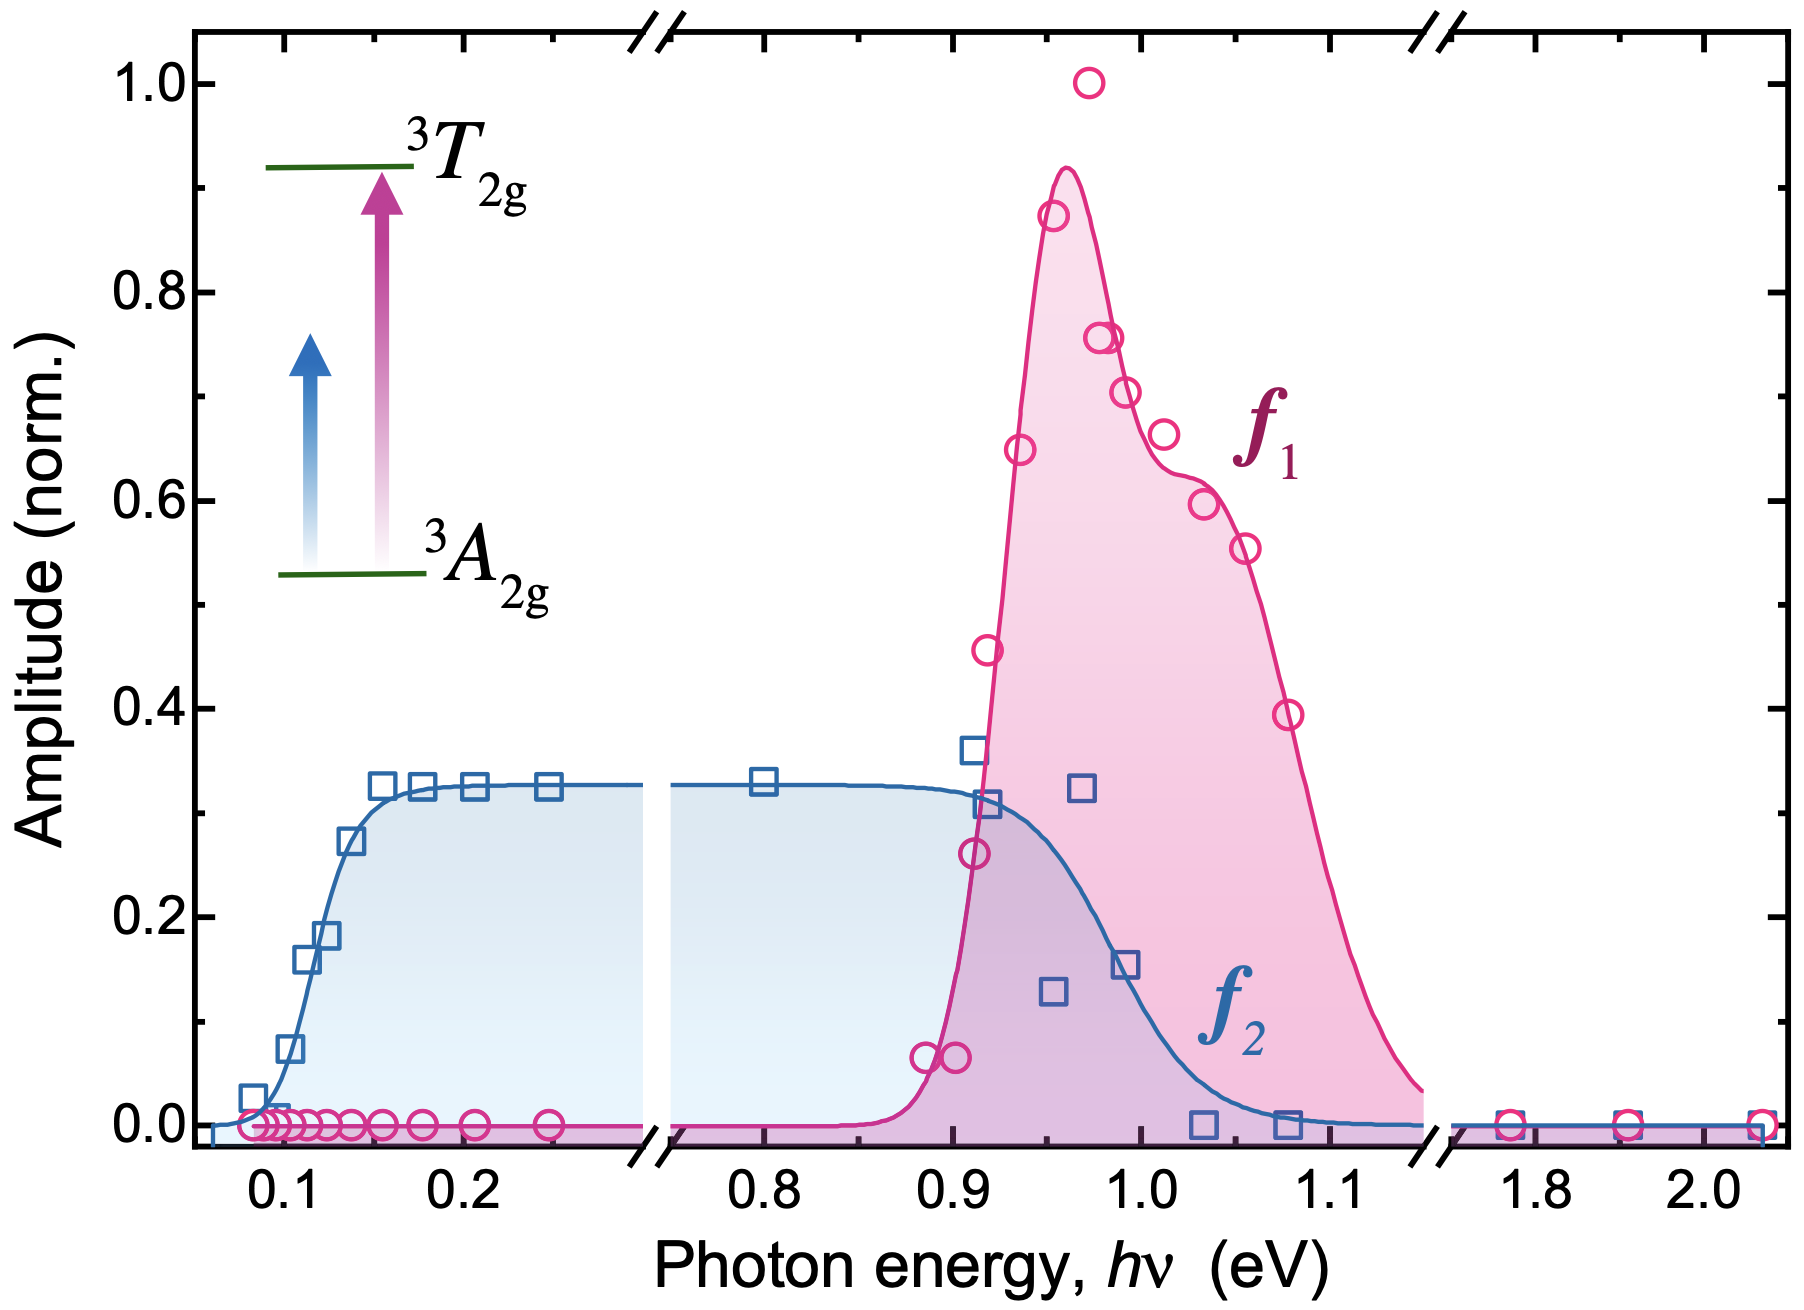
\includegraphics[width=\textwidth]{pictures/9.png}
        \caption{}
        \label{fig:9}
    \end{subfigure}
    \hspace{0.3cm}
    \begin{subfigure}[b]{0.28\textwidth}
        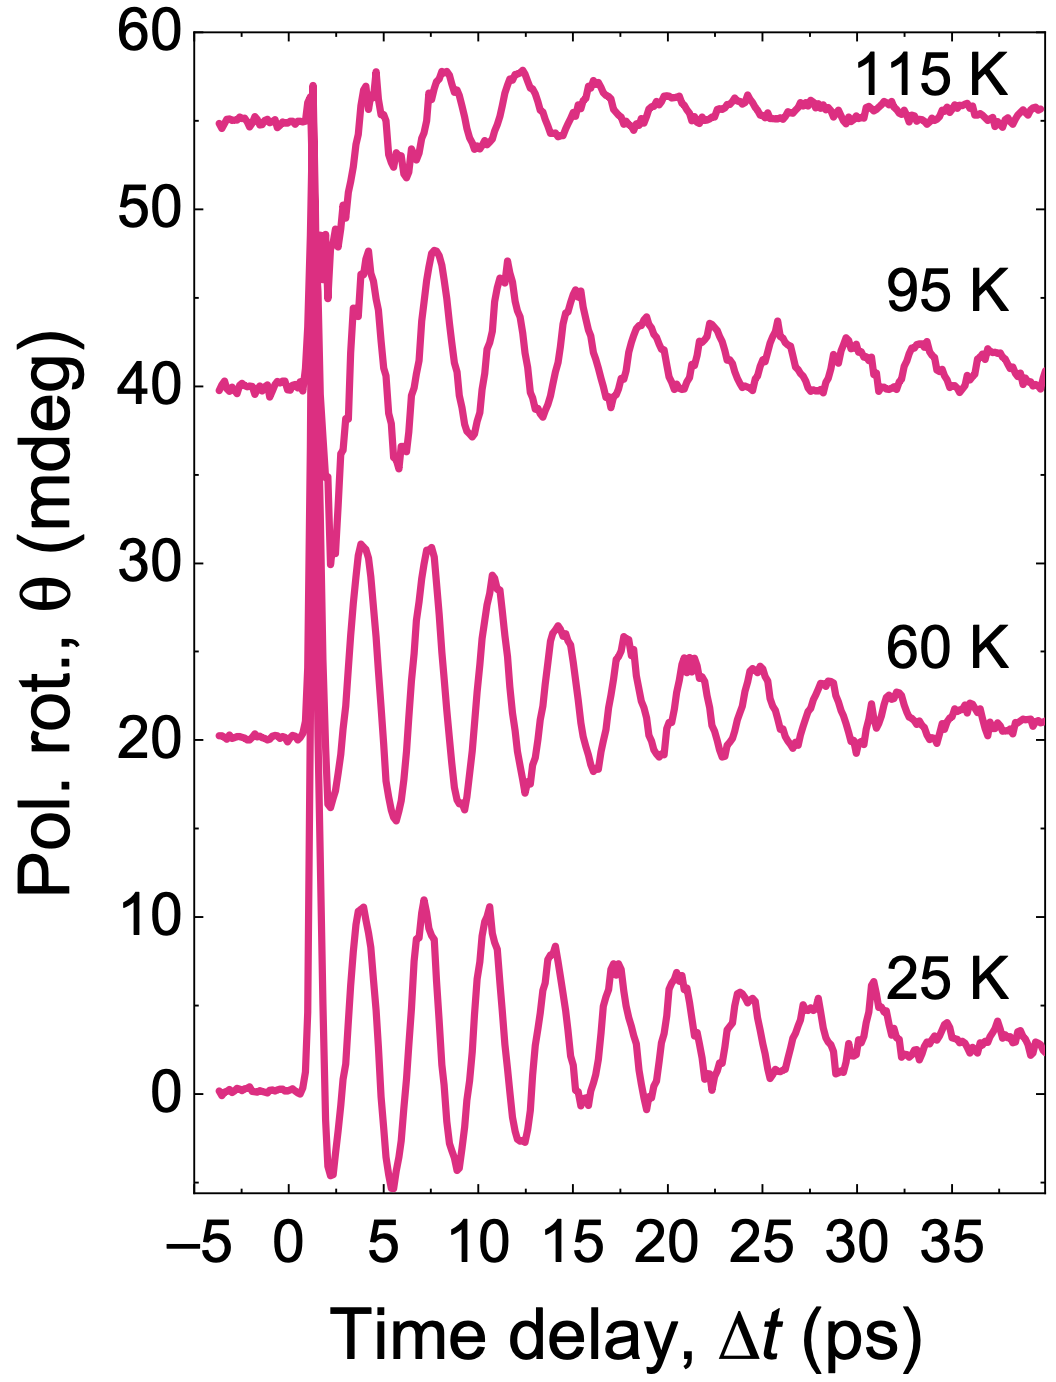
\includegraphics[width=\textwidth]{pictures/10.png}
        \caption{}
        \label{fig:10}
    \end{subfigure}
    \caption{\textbf{a)} The spectral dependencies of the amplitudes of the in-plane $f_1$ mode and the out-of-plane $f_2$ mode normalized to the maximum value of the $f_1$ mode. The solid lines are guides to the eye. \textbf{b)} The time-resolved rotation of polarization after pumping with an energy of \qty{1.08}{eV} at different temperatures. Both taken from \cite{afanasiev_controlling_2021}}
\end{figure}
\FloatBarrier
First, an effort was undertaken to reproduce one of the already established results from that paper.
Namely, to detect the in-plane magnon mode with a frequency of \qty{0.3}{THz} while pumping at \qty{1.08}{eV} and probing at \qty{800}{nm} which is shown for different temperatures in \autoref{fig:10}.
\begin{figure}[ht]
    \centering
    \includegraphics{pictures/plots/NiPS3_no_magnons.pdf} \vspace{-0.3cm}
    \caption{The measurement taken on the NiPS3 flake at a \qty{1.09}{eV} or \qty{1136}{nm} pump show no oscillations in the rotation of polarization or the transient reflectivity after \qty{23}{ps} after the zero-delay.}
    \label{fig:NiPS3_no_magnons}
\end{figure}
\FloatBarrier
\autoref{fig:NiPS3_no_magnons} shows a time trace of the rotation of polarization until \qty{23}{ps} after a \qty{1.09}{eV} pump.
There are no oscillations visible.
The measurements were done at different polarization directions for the pump and the probe pulse and at varying fluences, but still no fluctuations appeared.
In contrast to \cite{afanasiev_controlling_2021}\cite{toyoda_phase_2023} the measurements were not taken in transmission but in reflection.
Subsequent measurements using a magnetic field of up to \qty{2}{T}, to cant the spins more into the direction of the c-axis for an easier detection, show slight oscillations which only start after about \qty{30}{ps}.
It is possible, that the in-plane mode is first masked by the thermal demagnetization and then by the dominant GHz-modes decribed in the following.

Observing a longer timescale of around \qty{300}{ps} with the probe set to \qty{800}{nm} reveals two GHz-modes with the frequencies 13 and \qty{28}{GHz} which are labeled low-frequency (LFM) and high-frequency (LFM) mode, analogous to the two modes in NiO.
These modes are not yet described in literature.
Instead of fitting the oscillations, the easier method of FFT was used as the phase does not seem to change in the evaluated dependencies and only the amplitude and frequency are of importance to us.
It should be noted that the frequencies do not change from their values during the three measured dependencies and are therefore omitted from the following sections.

\subsection{Pump polarization dependence}
To help us understand the excitation mechanism behind the GHz-modes a pump polarization dependence is carried out.
For this purpose the rotation of polarization and the transient reflectivity was analyzed while changing the angle from 0° to 180° with a stepsize of 15°.
The probe polarization angle was set to 150° for the duration of this dependence.
Employing an FFT the amplitude along with the frequency of the detected oscillation are extracted.
A beating of two different oscillations is clearly visible in \autoref{fig:NiPS3_pump_polarization_dependence_diff}.
\begin{figure}[hbt!]
    \centering
    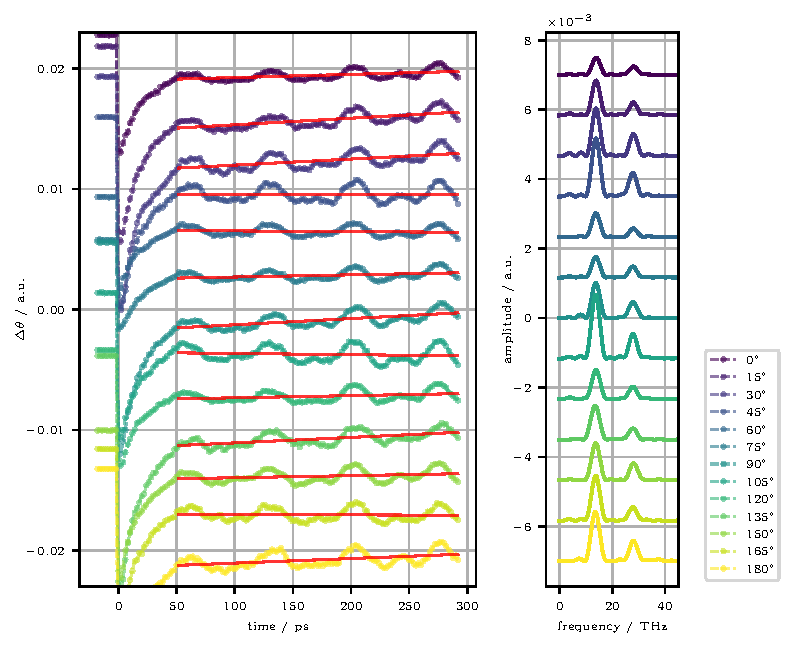
\includegraphics{pictures/plots/NiPS3_pump_polarization_dependence_diff.pdf} \vspace{-0.3cm}
    \caption{\textbf{a)} Rotation of polarization as a function of time taken at pump polarization angles ranging from 0° to 180° with a stepsize of 15°. The red lines depict the linear background. \textbf{b)} The FFTs of the traces at the different pump polarization angles display two prominent modes at \qty{13}{GHz} (LFM) and \qty{28}{GHz} (HFM).}
    \label{fig:NiPS3_pump_polarization_dependence_diff}
\end{figure}
\FloatBarrier
\begin{figure}[hbt!]
    \centering  
    \includegraphics{pictures/plots/NiPS3_pump_polarization_dependence_diff_ampl.pdf} \vspace{-0.3cm}
    \caption{The extracted amplitudes of the lf- and hf-mode in the rotation of polarization plotted against the pump polarization angle and normalized to the maximum value. The data traces were taken at a probe polarization of 150°. The continuous lines show the sinusoidal fit which yields a 3-fold symmetry.}
    \label{fig:NiPS3_pump_polarization_dependence_diff_ampl}
\end{figure}
\FloatBarrier
Considering the dependence in \autoref{fig:NiPS3_pump_polarization_dependence_diff_ampl}, a clear sinusoidal shape with a period of 60° be seen.
It is hard to determine to what crystallographic directions the angles of the orientation of polarization correspond to, as no literature on these modes is available yet, their origin is ambiguous and no dependencies of known features were done to identify the orientation of the sample in relation to our setup.
Nonetheless, the 3-fold symmetry of both modes is recognizable which indicates their origin to be associated with the 2D-lattice of the Ni$^{2+}$-ions as the honeycomb structure has the same symmetry.

The transient reflectivity in \autoref{fig:NiPS3_pump_polarization_dependence_sum} shows only one distinct mode, the hf-mode, as do all following transient reflectivity measurements.
As the transient reflectivity is regarded as a measure for non-magnetic dynamics this indicates that the hf-mode emerges from lattice dynamics.
The amplitude of the hf-mode in the transient reflectivity in \autoref{fig:NiPS3_pump_polarization_dependence_sum_ampl} also displays a 3-fold symmetry in regard to the pump polarization.
Furthermore, the same periodicities in the pump polarization dependencies for the rotation of polarization and transient reflectivity suggest that both the modes have a common origin.
Both polarization dependencies show some data points deviating from the sinusoidal shape in the region of 140°, implying some issues arising from the setup.
A possible explanation could be that the $\frac{\lambda}{2}$-plate used to adjust the polarization angle has a faulty spot.
As the pump does not hit the waveplate exactly in the middle, a change of angle would change the spot where the pump meets plate.
Aside from that, the other points fit into the shape quite well.
\begin{figure}[hbt!]
    \centering
    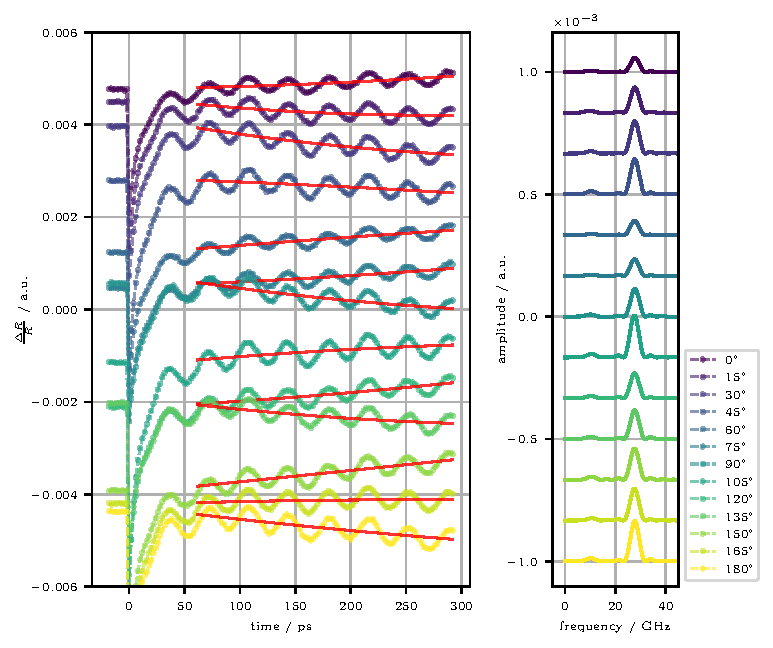
\includegraphics{pictures/plots/NiPS3_pump_polarization_dependence_sum.pdf} \vspace{-0.3cm}
    \caption{\textbf{a)} Transient reflectivity as a function of time taken at pump polarization angles ranging from 0° to 180° with a stepsize of 15°. The red lines depict the linear background. \textbf{b)} The FFTs of the traces at the different pump polarization angles display one prominent mode at \qty{28}{GHz}.}
    \label{fig:NiPS3_pump_polarization_dependence_sum}
\end{figure}
% \FloatBarrier
\begin{figure}[hbt!]
    \centering  
    \includegraphics{pictures/plots/NiPS3_pump_polarization_dependence_sum_ampl.pdf} \vspace{-0.3cm}
    \caption{The extracted amplitudes of the hf-mode in the transient reflectivity plotted against the pump polarization angle and normalized to the maximum value. The data traces were taken at a probe polarization of 150°. The continuous line shows the sinusoidal fit which yields a 3-fold symmetry.}
    \label{fig:NiPS3_pump_polarization_dependence_sum_ampl}
\end{figure}
\FloatBarrier

\newpage
\subsection{Probe polarization dependence}
The probe polarization dependence analyzed in this chapter makes a statement about the detection mechanism behind the oscillations we observe in the rotation of polarization seen in \autoref{fig:NiPS3_probe_polarization_dependence_diff}a.
For the following measurements the pump polarization angle was set to 180° and the probe polarization angle was varied from 0° to 180° with a stepsize of 15°.
As for the detection mechanism two magneto-optical effects come into question:
The magneto-optical Kerr effect (MOKE) which originates from a possible out-of-plane magnetization component and the Cotton-Mouton effect originating from an in-plane component of the Neél vector causing linear birefringence.
The Faraday effect does not depend on the polarization angle of the probe \cite{toyoda_phase_2023}.
Using the same procedure as for the pump polarization dependence, the amplitudes of the oscillations in \autoref{fig:NiPS3_probe_polarization_dependence_diff} are extracted via FFT.
\autoref{fig:NiPS3_probe_polarization_dependence_diff_ampl} portrays the amplitudes of both the lf- and hf-mode as a function of the probe polarization angle.
The continous lines display sinusoidal fits.
Taking the angle dependence in \autoref{fig:NiPS3_probe_polarization_dependence_diff_ampl} into account, the conclusion can be drawn that the observed signal stems from linear birefringence, as theory also suggests that such a 2-fold symmetry corresponds to linear birefringence \cite{satoh_excitation_2017}.
It is also visible that the amplitude completely vanishes at the minima of the sinusoidal curve.
\begin{figure}[hbt!]
    \centering
    \includegraphics{pictures/plots/NiPS3_probe_polarization_dependence_diff.pdf} \vspace{-0.3cm}
    \caption{\textbf{a)} Rotation of polarization as a function of time taken at probe polarization angles ranging from 0° to 180° with a stepsize of 15°. The red lines depict the linear background. \textbf{b)} The FFTs of the traces at the different probe polarization angles display two prominent modes at \qty{13}{GHz} and \qty{28}{GHz}.}
    \label{fig:NiPS3_probe_polarization_dependence_diff}
\end{figure}
% \FloatBarrier
\begin{figure}[hbt!]
    \centering  
    \includegraphics{pictures/plots/NiPS3_probe_polarization_dependence_diff_ampl.pdf} \vspace{-0.3cm}
    \caption{The extracted amplitudes of the lf- and hf-mode in the rotation of polarization plotted against the probe polarization angle and normalized to the maximum value. The data traces were taken at a pump polarization of 180°. The continuous lines show the sinusoidal fit which yields a 2-fold symmetry.}
    \label{fig:NiPS3_probe_polarization_dependence_diff_ampl}
\end{figure}
\FloatBarrier
\autoref{fig:NiPS3_probe_polarization_dependence_diff} shows the measured transient reflectivity for the different probe polarization angles together with the respective FFT which again only yields the hf-mode.
The probe polarization dependence of the transient reflectivity plotted in \autoref{fig:NiPS3_probe_polarization_dependence_sum_ampl} displays the same periodicity as the rotation of polarization.
\begin{figure}[hbt!]
    \centering
    \includegraphics{pictures/plots/NiPS3_probe_polarization_dependence_sum.pdf} \vspace{-0.3cm}
    \caption{\textbf{a)} Transient reflectivity as a function of time taken at probe polarization angles ranging from 0° to 180° with a stepsize of 15°. The red lines depict the quadratic background. \textbf{b)} The FFTs of the traces at the different probe polarization angles display one prominent mode at \qty{28}{GHz}.}
    \label{fig:NiPS3_probe_polarization_dependence_sum}
\end{figure}
% \FloatBarrier
\begin{figure}[hbt!]
    \centering  
    \includegraphics{pictures/plots/NiPS3_probe_polarization_dependence_sum_ampl.pdf} \vspace{-0.3cm}
    \caption{The extracted amplitudes of the hf-mode in the transient reflectivity plotted against the probe polarization angle and normalized to the maximum value. The data traces were taken at a pump polarization of 180°. The continuous line shows the sinusoidal fit which yields a 2-fold symmetry.}
    \label{fig:NiPS3_probe_polarization_dependence_sum_ampl}
\end{figure}
\FloatBarrier

\subsection{Temperature dependence}
The temperature dependence was measured to be able to determine whether the two modes are of magnetic or non-magnetic origin.
The pump and probe polarizations were set to 180° and 150°, as this combination of angles yielded the smoothest oscillations.
The temperature was varied from 77 to \qty{170}{K} with a stepsize of \qty{10}{K} except around the Neél temperature (\qty{155}{K}), where the stepsize was reduced to \qty{5}{K}.
What we see now in \autoref{fig:NiPS3_temp_dependence_diff} is that both modes completely vanish above a certain temperature.
For the lf-mode this temperature coincides with the Neél temperature, which proves a connection to the magnetic system.
For the hf-mode whose detected amplitude is always smaller than the one from the lf-mode, any noticeable amplitude value vanishes after around \qty{120}{K}.
\begin{figure}[hbt!]
    \centering
    \includegraphics{pictures/plots/NiPS3_temp_dependence_diff.pdf} \vspace{-0.3cm}
    \caption{\textbf{a)} Rotation of polarization as a function of time acquired at temperatures ranging from 77 to \qty{170}{K} with an approximate stepsize of \qty{10}{K}. The blue lines depict the linear background. \textbf{b)} The FFTs of the traces at the different temperatures display two prominent modes at \qty{13}{GHz} and \qty{28}{GHz} which both vanish at two distinct temperatures.}
    \label{fig:NiPS3_temp_dependence_diff}
\end{figure}
% \FloatBarrier
\begin{figure}[hbt!]
    \centering  
    \includegraphics{pictures/plots/NiPS3_temp_dependence_diff_ampl.pdf} \vspace{-0.3cm}
    \caption{The exctracted amplitudes of the lf-mode in the rotation of polarization plotted against the temperatures, the respective data traces were taken at. A vanishing of the amplitudes after the Neél temperature is observed.}
    \label{fig:NiPS3_temp_dependence_diff_ampl}
\end{figure}
\FloatBarrier
As the transient reflectivity reflects the lattice dynamics, the amplitudes are not expected to be temperature dependent.
This is supported by the amplitude values of the hf-mode in \autoref{fig:NiPS3_temp_dependence_sum_ampl} being random, not following any trend and persisting even after the Neél temperature.
It can be concluded that the hf-mode originates in the lattice.
It couples to the magnetic system and induces dynamics which scale with the magnetic order.
\begin{figure}[hbt!]
    \centering
    \includegraphics{pictures/plots/NiPS3_temp_dependence_sum.pdf} \vspace{-0.3cm}
    \caption{\textbf{a)} Transient reflectivity as a function of time acquired at temperatures ranging from 77 to \qty{170}{K} with an approximate stepsize of \qty{10}{K}. The blue lines depict the linear background. \textbf{b)} The FFTs of the traces at the different temperatures display one prominent mode at \qty{28}{GHz}.}
    \label{fig:NiPS3_temp_dependence_sum}
\end{figure}
% \FloatBarrier
\begin{figure}[hbt!]
    \centering  
    \includegraphics{pictures/plots/NiPS3_temp_dependence_sum_ampl.pdf} \vspace{-0.3cm}
    \caption{The exctracted amplitudes of the hf-mode in the transient reflectivity plotted against the temperatures, the respective data traces were taken at. There is no clear trend visible.}
    \label{fig:NiPS3_temp_dependence_sum_ampl}
\end{figure}
\FloatBarrier



% \chapter{Abbildungen und Tabellen}

\section{Abbildungen}

Achten Sie bei ihren Plots auf ausreichend große Achsenbschriftungen, ausreichende Schriftdicken und gut unterscheidbare Farben.
Im Idealfall haben Sie im Plot und der Arbeit die gleiche Schriftgröße und Schriftart.
Dies lässt sich durch Erstellen des Plots in der korrekten Größe und Einbinden mit dem optionalen Argument \texttt{scale=1} erreichen. Ein Beispiel sehen Sie in Abbildung \ref{fig:bsp}.

Nutzen Sie wenn möglich Vektorgrafiken (pdf) und nur in Ausnahmen Rastergrafiken wie .png oder .jpg.
Setzen Sie Punkte hinter Abbildungsunterschriften.

\begin{figure}
    \centering
    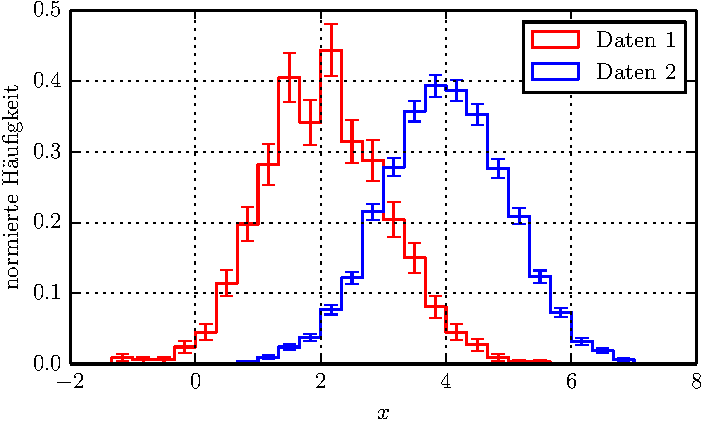
\includegraphics[scale=1]{./Plots/Histogramm.pdf}
    \caption{Ein Histogramm mit Fehlerbalken für zwei Datensätze, Schriftgröße und -art entsprechen der des Dokuments.}
    \label{fig:bsp}
\end{figure}

\section{Tabellen}

Tabellen sollten so einfach wie möglich aufgebaut sein, verzichten Sie auf zu viele Linien. In fast allen Fällen reichen drei horizontale Linien aus, jeweils über und unter der Tabelle und zwischen den Spaltenüberschriften und der eigentlichen Tabelle.

Das Paket \texttt{booktabs} stellt hierfür \verb_\toprule_, \verb_\midrule_ und 
\verb_\bottomrule_ zur Verfügung.
Das Paket \texttt{siunitx} stellt eine extrem mächtige neue Spalteneinstellung bereit: \texttt{S}, mit ihr können Zahlen und Einheiten sehr sauber und gut ausgerichtet gesetzt werden.

Diese Vorlage geht von Tabellenüberschriften aus, möchten Sie dagegen Tabellenunterschriften entfernen Sie das entsprechende optionale Argument für die Dokumentenklasse in der Präambel.

Ein Beispiel ist Tabelle~\ref{tab:bsp}.
\begin{table}
    \centering
    \caption{Beispieltabelle mit willkürlichen Werten, für die Zahlenwerte wurde die S-Option aus \texttt{siunitx} verwendet.}
    \label{tab:bsp}
    \begin{tabular}{S[table-format=4.2] S[table-format=3.2]}
        \toprule
        {$p \mathrel{/} \si{\pascal}$}  & {$T \mathrel{/} \si{\kelvin}$} \\
        \midrule
        1024,23 & 273,15 \\
        1025,31 & 274,5 \\
        1026,27 & 276,2 \\
        \bottomrule
    \end{tabular}
\end{table}


% \appendix
% Hier beginnt der Anhang, nummeriert in lateinischen Buchstaben
% \chapter{Ein Anhangskapitel}

Hier könnte ein Anhang stehen, falls Sie z.\,B.\ Code, Konstruktionszeichnungen oder Ähnliches mit in die Arbeit bringen wollen.
Im Normalfall stehen jedoch alle Ihre Resultate im Hauptteil der Bachelorarbeit und ein Anhang ist überflüssig.


\backmatter
\printbibliography

% \cleardoublepage
% From https://www.tu-dortmund.de/studierende/im-studium/pruefungsangelegenheiten/allgemeine-vordrucke/
% 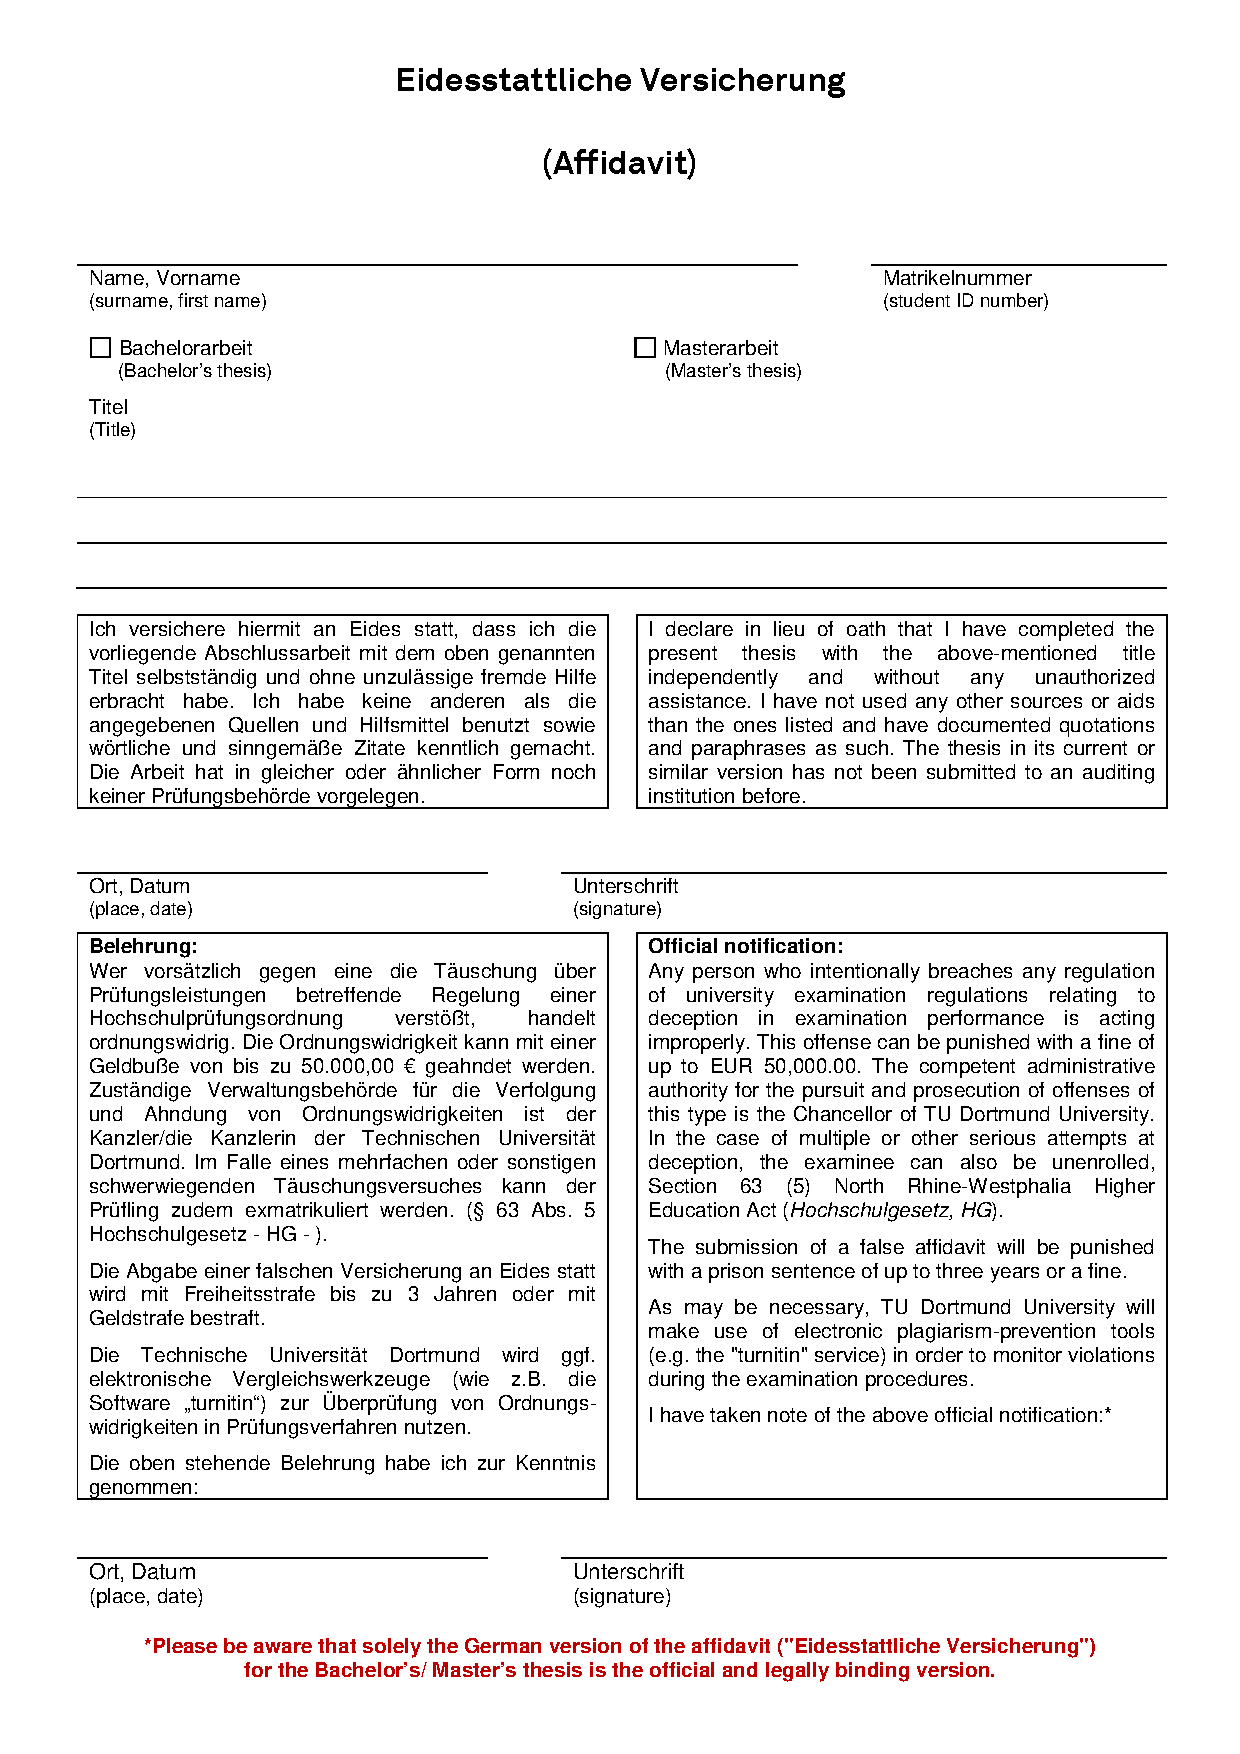
\includepdf{content/Eidesstattliche_Versicherung.pdf}

\end{document}
